\documentclass[pdftex,12pt,a4paper]{article}

\usepackage[turkish,english]{}
\usepackage{graphicx}  
\usepackage[margin=2.5cm]{geometry}
\usepackage{breakcites}
\usepackage{indentfirst}
\usepackage{pgfgantt}
\usepackage{pdflscape}
\usepackage{float}
\usepackage{epsfig}
\usepackage{epstopdf}
\usepackage[cmex10]{amsmath}
\usepackage{url}
\usepackage{stfloats}
\usepackage{multirow}

\renewcommand{\refname}{REFERENCES}
\linespread{1.3}

\usepackage{mathtools}
%\newcommand{\HRule}{\rule{\linewidth}{0.5mm}}
\thispagestyle{empty}
\begin{document}
\begin{titlepage}
\begin{center}
\textbf{}\\
\textbf{\Large{ISTANBUL TECHNICAL UNIVERSITY}}\\
\vspace{0.5cm}
\textbf{\Large{COMPUTER ENGINEERING DEPARTMENT}}\\
\vspace{2cm}
\textbf{\Large{BLG 242E\\ DIGITAL CIRCUITS LABORATORY\\ EXPERIMENT REPORT}}\\
\vspace{2.8cm}
\begin{table}[ht]
\centering
\Large{
\begin{tabular}{lcl}
\textbf{EXPERIMENT NO}  & : & 1 \\
\textbf{EXPERIMENT DATE}  & : & 15.02.2019 \\
\textbf{LAB SESSION}  & : & FRIDAY - 14.00 \\
\textbf{GROUP NO}  & : & G13 \\
\end{tabular}}
\end{table}
\vspace{1cm}
\textbf{\Large{GROUP MEMBERS:}}\\
\begin{table}[ht]
\centering
\Large{
\begin{tabular}{rcl}
{
150180704  & : & C\.{I}HAT AKK\.{I}RAZ \\
150180707  & : & FAT\.{I}H ALTINPINAR \\
150180734  & : & S\.{I}NAN \c{S}AR \\
}
\end{tabular}}
\end{table}
\vspace{2.8cm}
\textbf{\Large{SPRING 2019}}

\end{center}

\end{titlepage}

\newpage

\thispagestyle{empty}
\centering{\LARGE{ \textbf{ETHIC FORM}}}\\
\centering{\LARGE{\textbf{for}}}\\
\centering{\LARGE{\textbf{BLG242E Logic Circuits Laboratory}}}\\[0.2cm]
As a student of \\Istanbul Technical University Faculty of Computer and Informatics Engineering;
\begin{enumerate}
    \item I will not attempt to cheat in quizes and final exam,
    \item I will not use disallowed sources or tools (mobile phone, calculator etc.) during the exam,
    \item I will not write any information (formula, text, figure etc.) on the table, sheets or books that are allowed to be used during the exam,
    \item I will give reference when using printed or online published sources,
    \item I will not use the results in a source as they are, or by changing a part of them without giving a reference,
    \item I will not show unused sources as used, 
    \item I will not present someone else’s idea as my own idea, 
    \item I will not make someone do my homework, project or thesis for money or anything else,
    \item I will not take an exam or enter a lecture on behalf of others,
    \item I will not make excuses for not attending in exams or lessons by taking reports from someone I know (medical doctor parents or relatives),
    \item I will refrain from deliberately harming the public materials at our university,  
    \item I will comply with the safety rules in laboratory work,
    \item I will behave in accordance with the rules of respect for the lecturers and teaching assistants
\end{enumerate}
\vspace{-1em}
\centering{\LARGE{signed by}}\\
\vspace{-1em}
\begin{table}[ht]
\centering
\begin{tabular}{rcl}
150180704  & : & C\.{I}HAT AKK\.{I}RAZ \\
150180707  & : & FAT\.{I}H ALTINPINAR \\
150180734  & : & S\.{I}NAN \c{S}AR \\
\end{tabular}
\end{table}
\vspace{-1em}
 \begin{table}[ht]
 \begin{tabular}{lr}
%\textbf{Date:\hspace*{1.0cm}/\hspace*{1.0cm}/} &\qquad \qquad\qquad\qquad \qquad\qquad\qquad \qquad\qquad\qquad \qquad\qquad \textbf{SIGNED}\\
\end{tabular}
\end{table} % adds the ethic sign
\addcontentsline{toc}{section}{\numberline {}ETHICS}
\newpage

\thispagestyle{empty}
\addtocontents{toc}{\contentsline {section}{\numberline {}FRONT COVER}{}}
\addtocontents{toc}{\contentsline {section}{\numberline {}CONTENTS}{}}
\setcounter{tocdepth}{4}
\tableofcontents
\clearpage

\setcounter{page}{1}
\section{INTRODUCTION }

\begin{flushleft}
\paragraph{}
In this experiment, tests were performed with CADET, the function generator and oscilloscope. Aim of the experiments were learning the parts of CADET, how to use them. There were five parts of this experiment in total. Some of them required multiple circuits to be built.
% Detailed information about each part of the experiment is available in the following sections.
% Bence raporda boyle birsey yazmaya gerek yok.
\end{flushleft}
\section{REQUIREMENTS }

\begin{flushleft}
\underline{Tools Used}\cite{booklet}
\end{flushleft}
\begin{itemize}
    \item C.A.D.E.T
    \item Function Generator
    \item Oscilloscope
    \item 74000 series ICs
    \begin{itemize}
        \item 74x$x^{1}$04 - Hex Inverter
    \end{itemize}
\end{itemize}

\begin{flushleft}
\subsection{PART 1}
\end{flushleft}


\begin{figure}[ht]
	\centering
	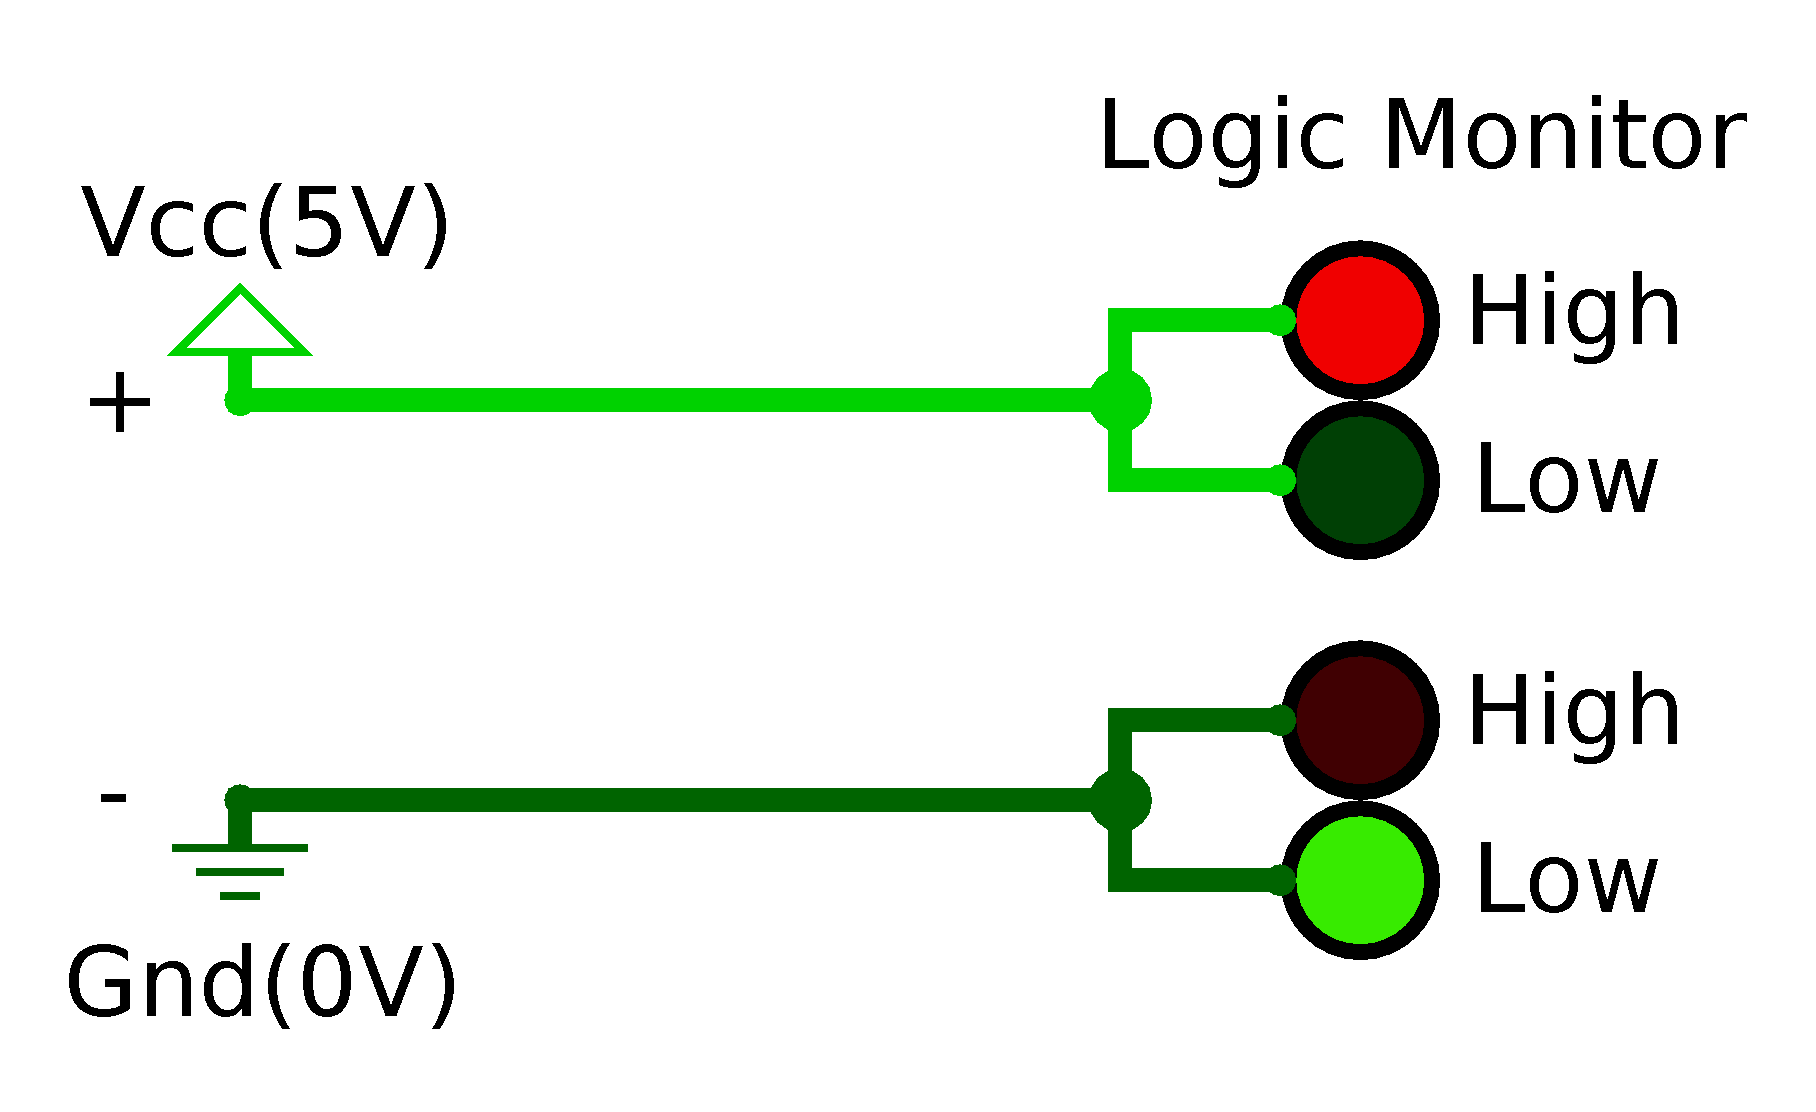
\includegraphics[width=0.5\textwidth]{part1_800.png}	
	\caption{Logic monitor revealing logic states of Vcc and Ground}
	\label{fig1}
\end{figure}
\begin{flushleft}
\paragraph{}
In the first part of the experiment, a simple circuit was created with the power distributor in CADET. 5 volt Vcc supply and GND (ground pin) were connected to different power strips on the breadboard. Then both power strips were connected to a logic monitor(a different monitor for each individual power strip). Logic monitor showed high voltage for Vcc source while it showed low voltage for ground as it can be seen in Figure 1.
\end{flushleft}

% \cite{ref1} how to cite

\begin{flushleft}
\subsection{PART 2}
\end{flushleft}

\begin{figure}[ht]
	\centering
	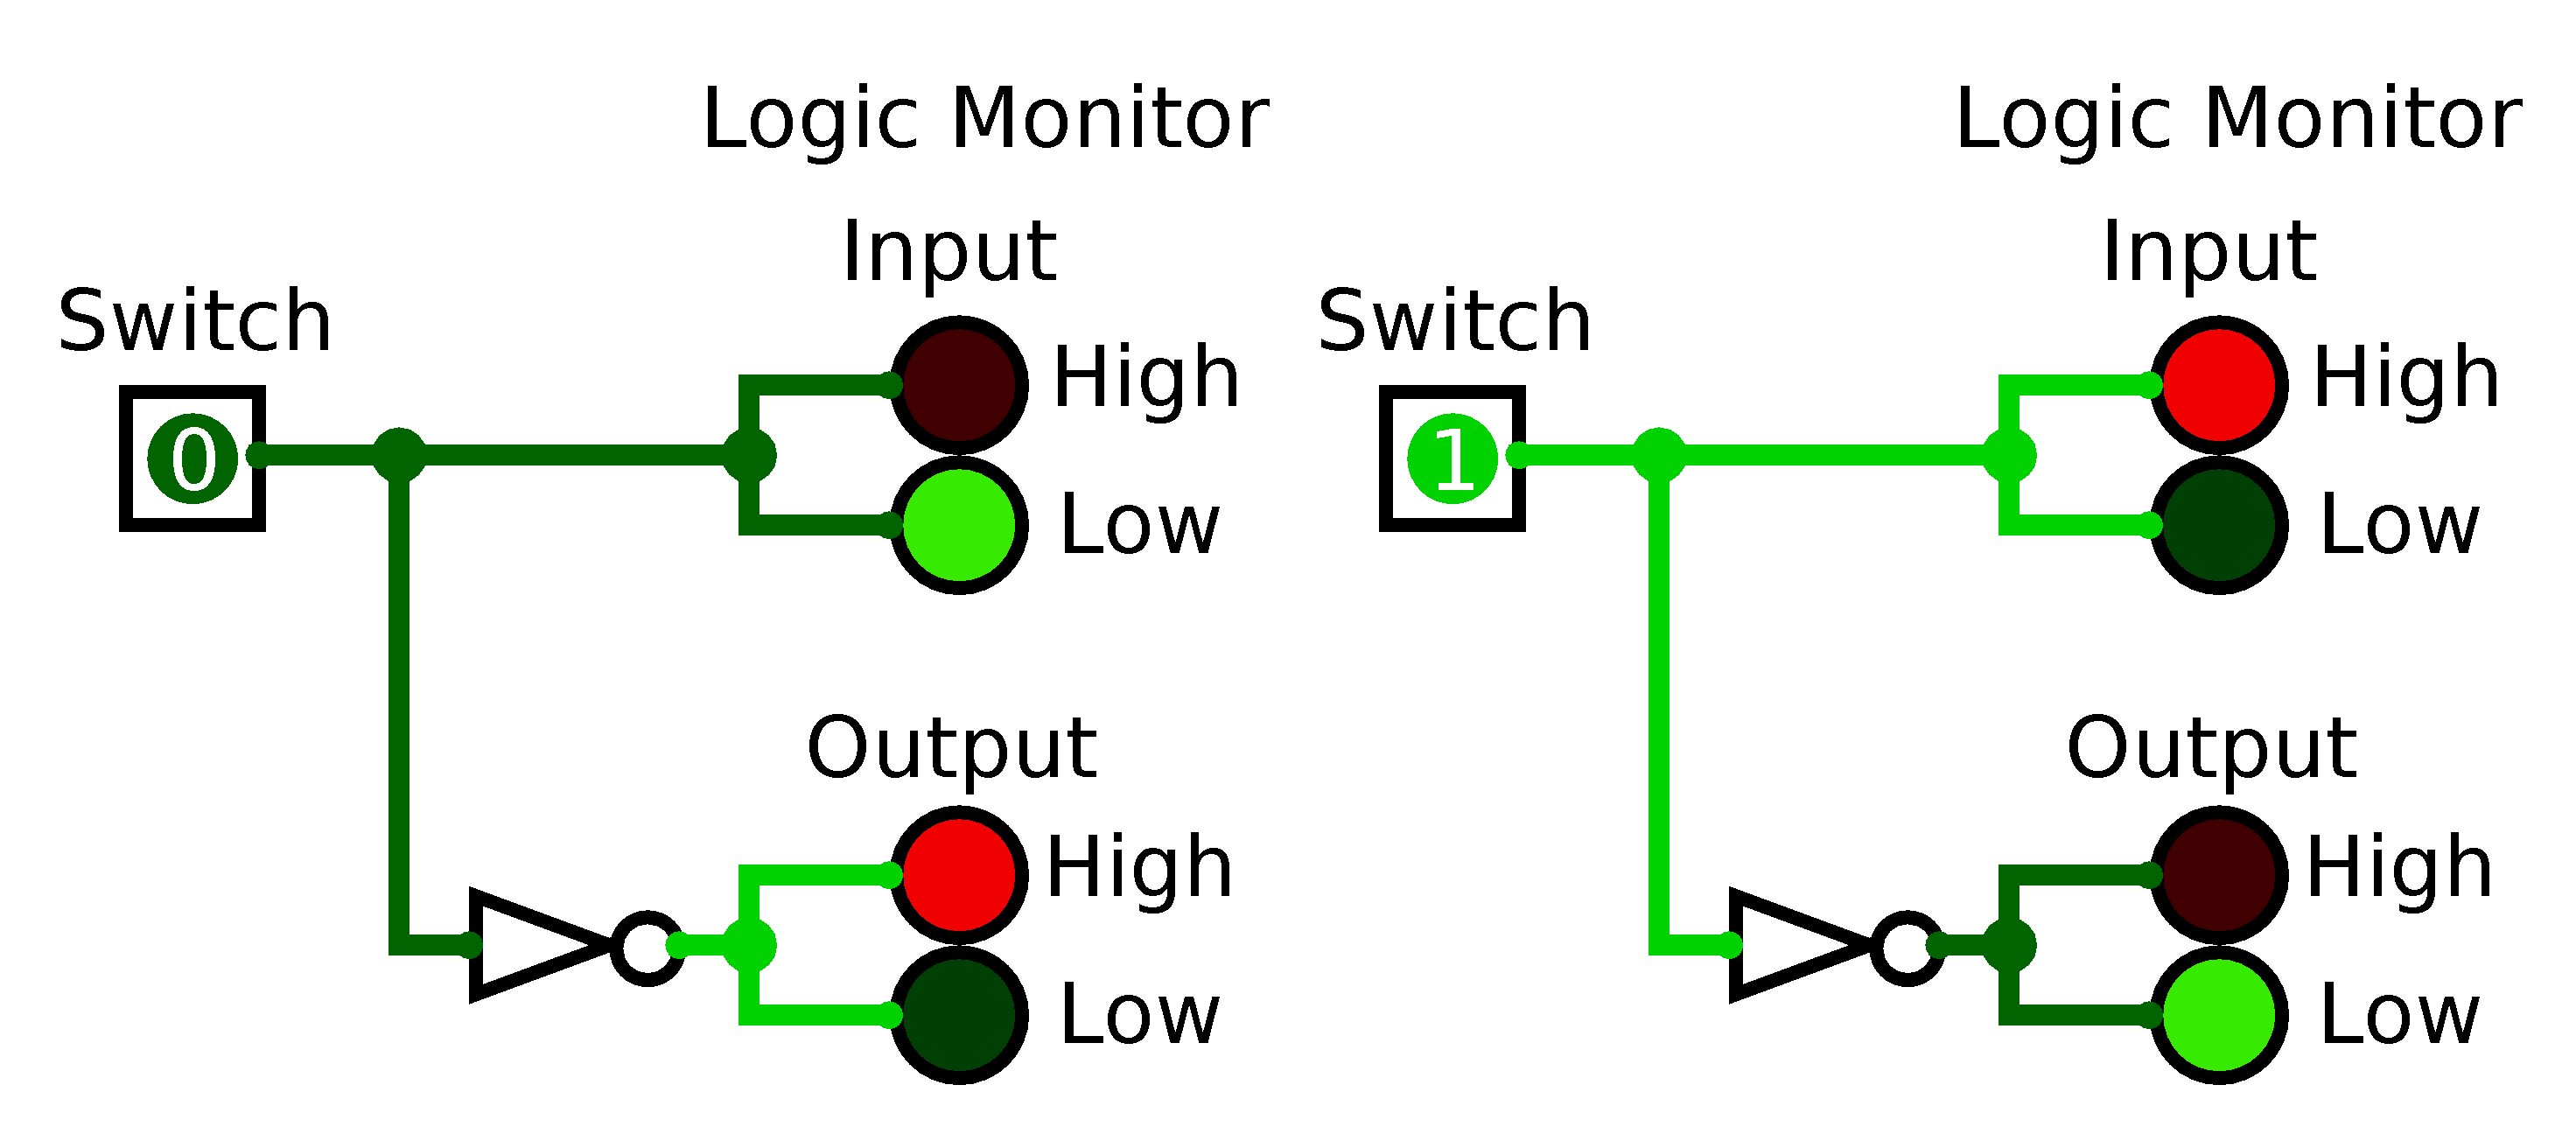
\includegraphics[width=0.5\textwidth]{part2_800.png}	
	\caption{Left: Switch is off, Right: Switch is on}
	\label{fig2}
\end{figure}

\begin{flushleft}
\paragraph{}
In the next part of the experiment, a circuit was designed to invert the input using the 7404 hex inverter. 5 volt Vcc supply was connected with the pin in the upper right corner and the Gnd voltage was applied to the pin in the lower left corner. Using Logic switches and SPDT switches, the input was changed and the status of the output on the logic monitor was observed. If the inverter is fed by a low logical signal, the output will be a high logical signal, if the output is fed by a high logical signal, the output will be a low logical signal. The difference between logic switches and SPDT switches used in the experiment can be explained quite simply. While the SPDT switches allow the user to control the input voltages, logic switches work on predetermined values of voltage(logic 1 and 0 having their respective values). Therefore SPDT switches allow the user to be more flexible and specific.
\end{flushleft}



\begin{flushleft}
\subsection{PART 3}
\end{flushleft}
\begin{flushleft}
\paragraph{}
Voltage values at GND(ground) and 5 volt Vcc were measured with the voltmeter function of the multimeter. 5V output was measured as 4.96 volts and GND was 0 volt. Resistance of the potentiometer was also measured with the multimeter and then was set to 8 K Ohms as it was required.
\end{flushleft}

\begin{flushleft}
\subsection{PART 4}
\end{flushleft}

\begin{figure}[ht]
	\centering
	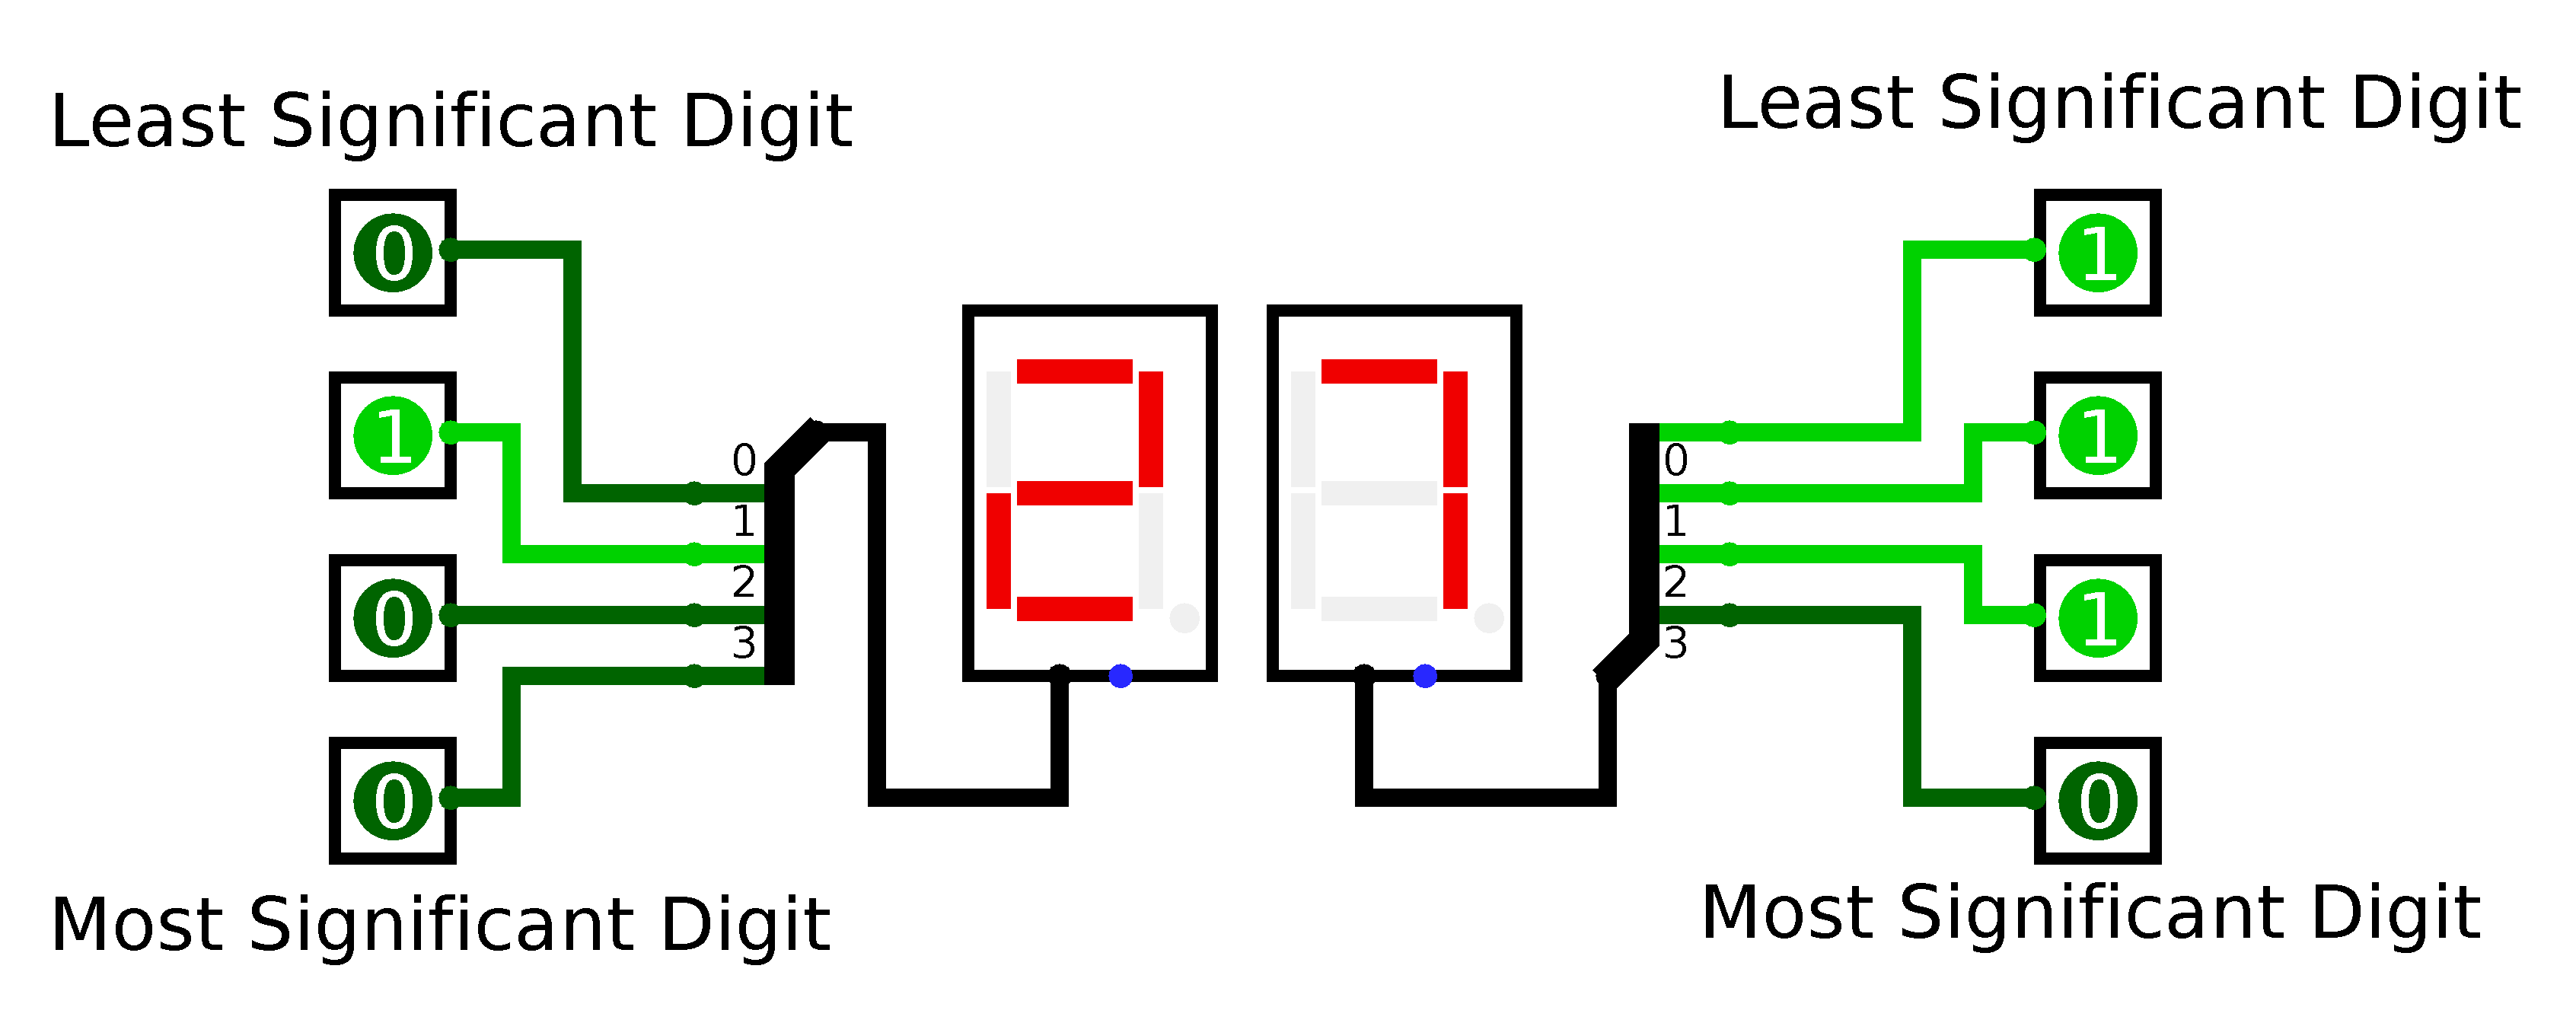
\includegraphics[width=0.75\textwidth]{part4_800.png}	
	% TODO:
	\caption{Displaying '27' with using binary coded decimal}
	% Binary coded decimal
	\label{fig3}
\end{figure}

\paragraph{}
\begin{flushleft}
The pins on the logic monitor were connected to the inputs in the display section, considering the most significant bits, the least significant bits and the order of bits. In order to display the number 27 in the display part, the input values from the pins have to be 0010 and 0111(2 and 7 in decimal). Each pin was set to 0 (closed) and 1 (open) position accordingly.

\end{flushleft}

\begin{flushleft}
\subsection{PART 5}
\end{flushleft}
\begin{flushleft}
\paragraph{}
In the last part of the experiment, it is required to create some waves with different properties and frequencies using the function generator, then displaying them on oscilloscope.

%In the last part of the experiment, various measurements were made using the function generator %and oscilloscope. Output type of the function generator(type of wave(sin, square,etc.) and it %being CMOS or TTL) was changed whenever is was necessary.
\end{flushleft}

\begin{flushleft}
\subsubsection{27 kHz TTL}
\begin{figure}[h]
    \centering
	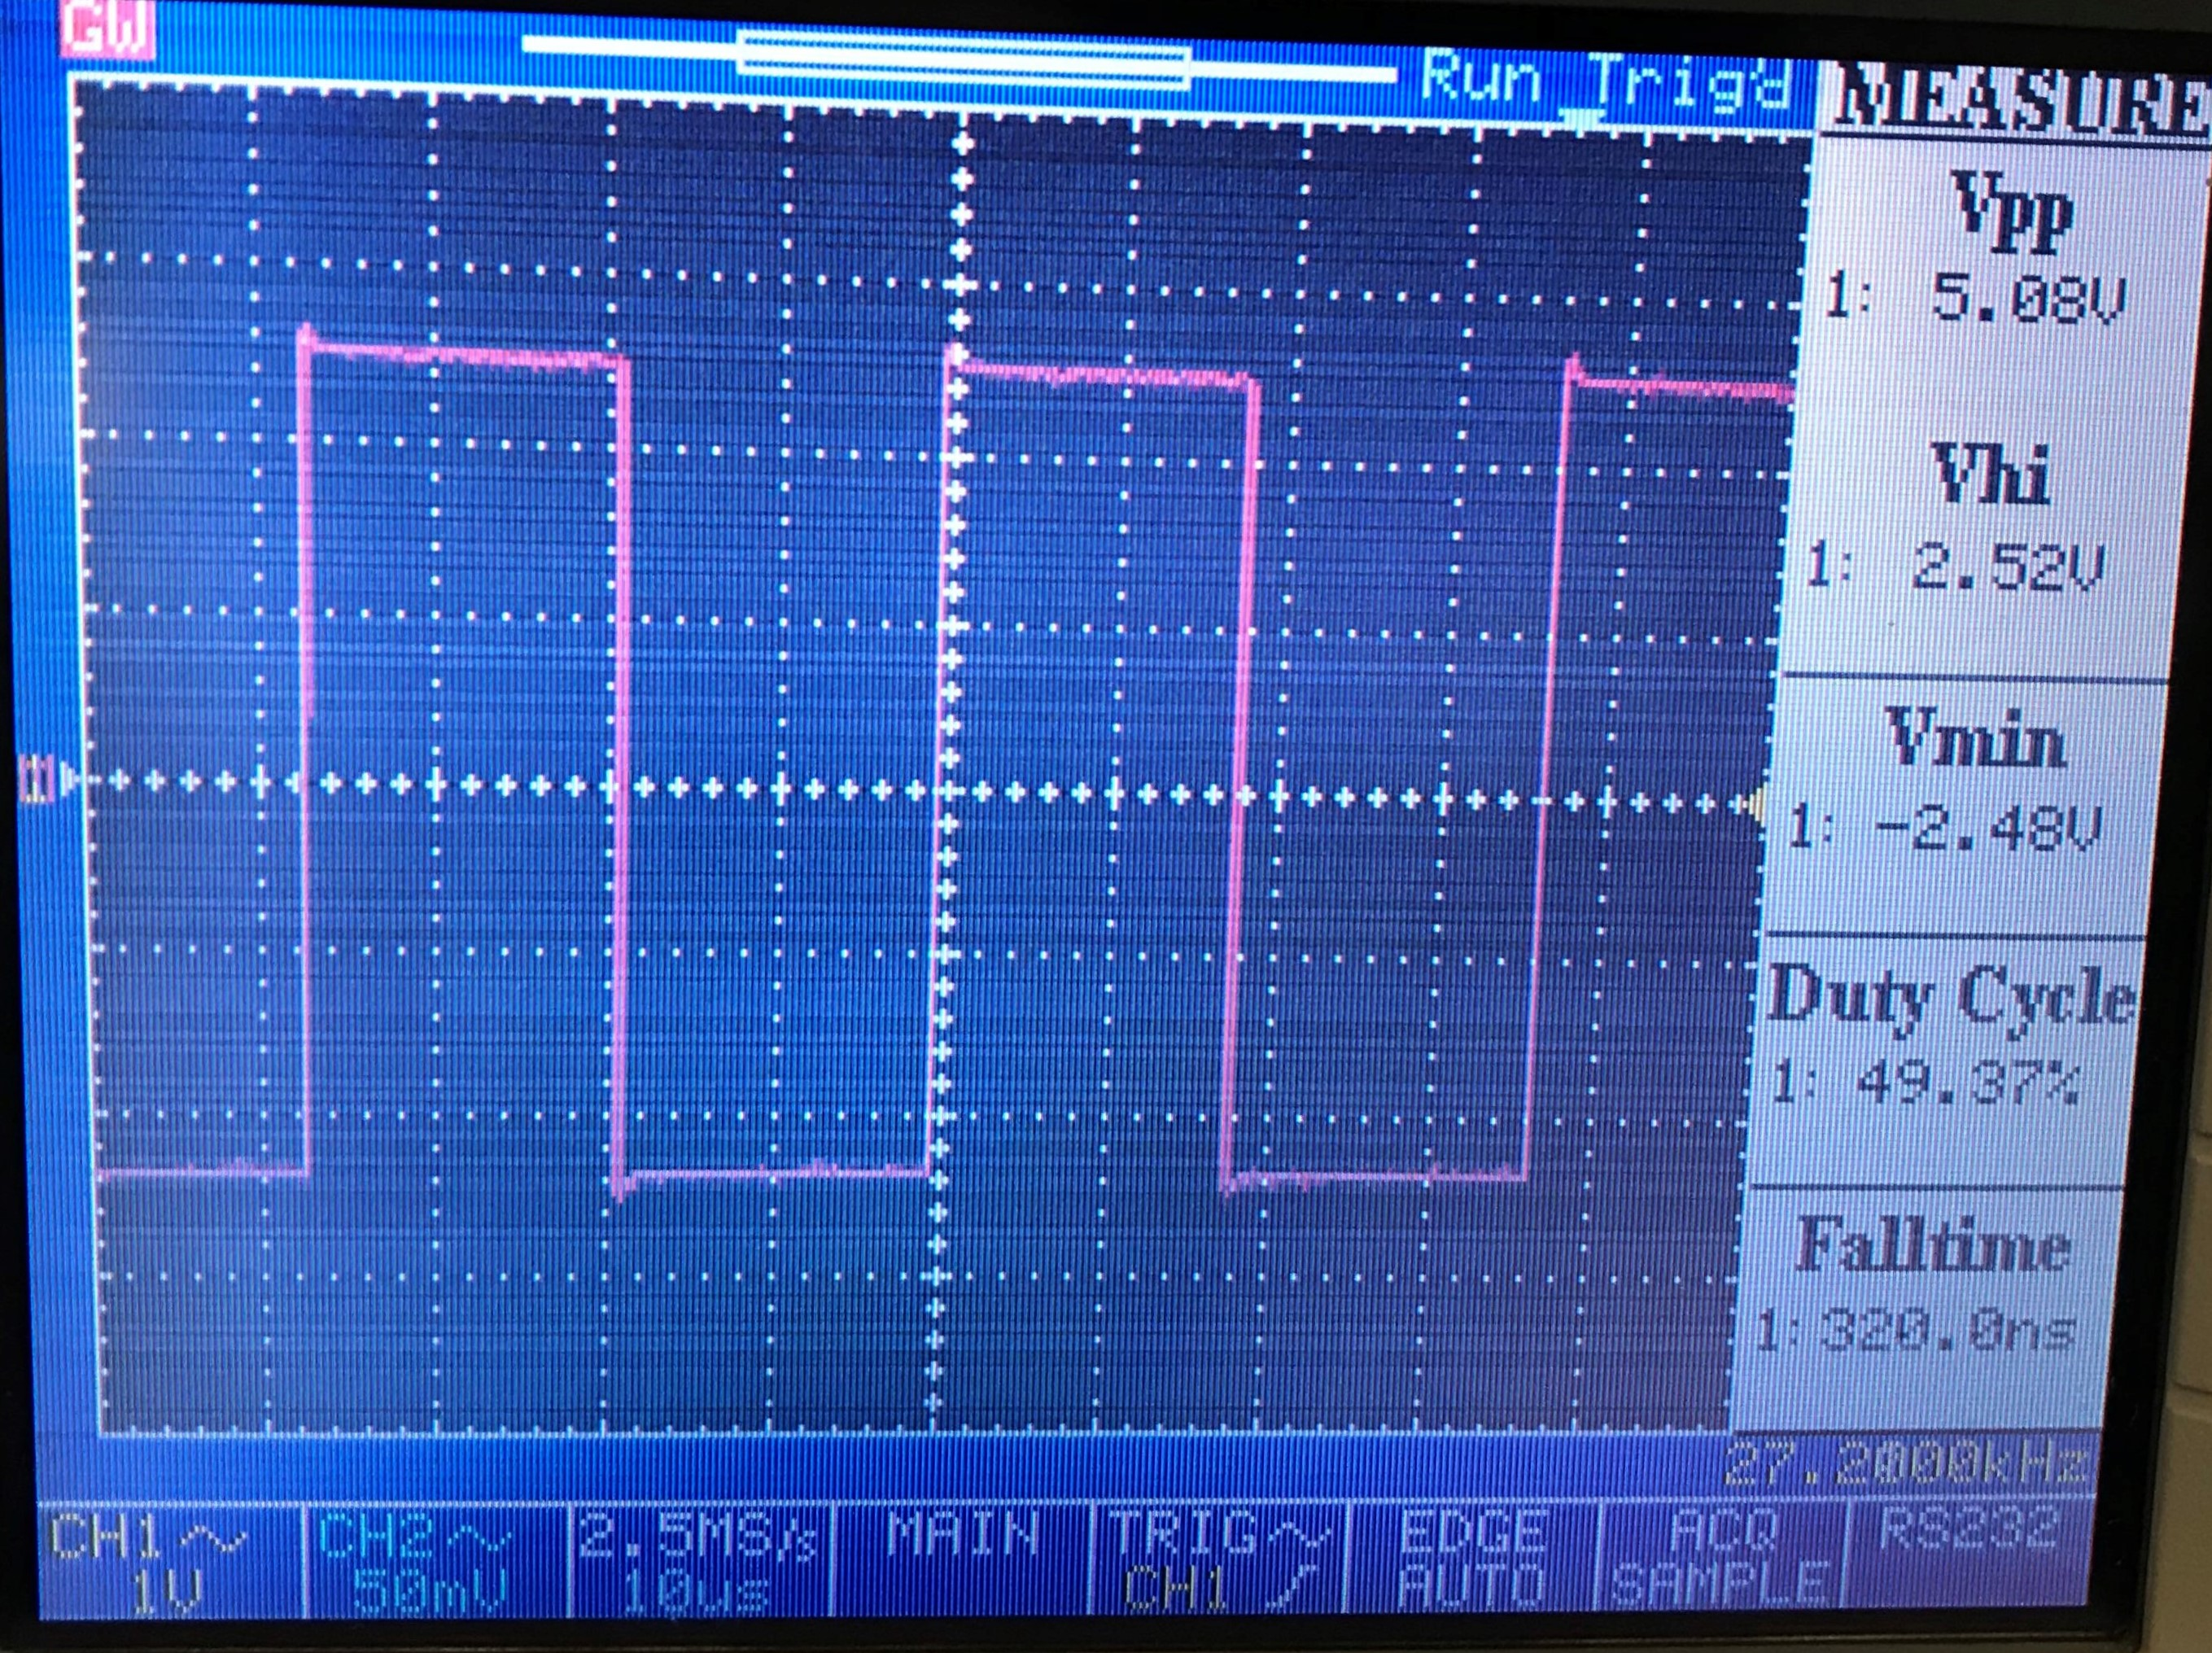
\includegraphics[width=0.5\textwidth]{Photos/5_1_closeup.jpg}
	\caption{27 kHz TTL}
	\label{fig4}
\end{figure}

\paragraph{}
In order to obtain 27kHz TTL input from the function generator, setting the range selector to 100k and adjusting 27kHz with the frequency slider were needed. Adjusting voltage output was not required since TTL always gives 5V square wave as output.
\end{flushleft}


\newpage
\begin{flushleft}
\subsubsection{5 V (Vpp), 1992 Hz CMOS}
\begin{figure}[h]
    \centering
	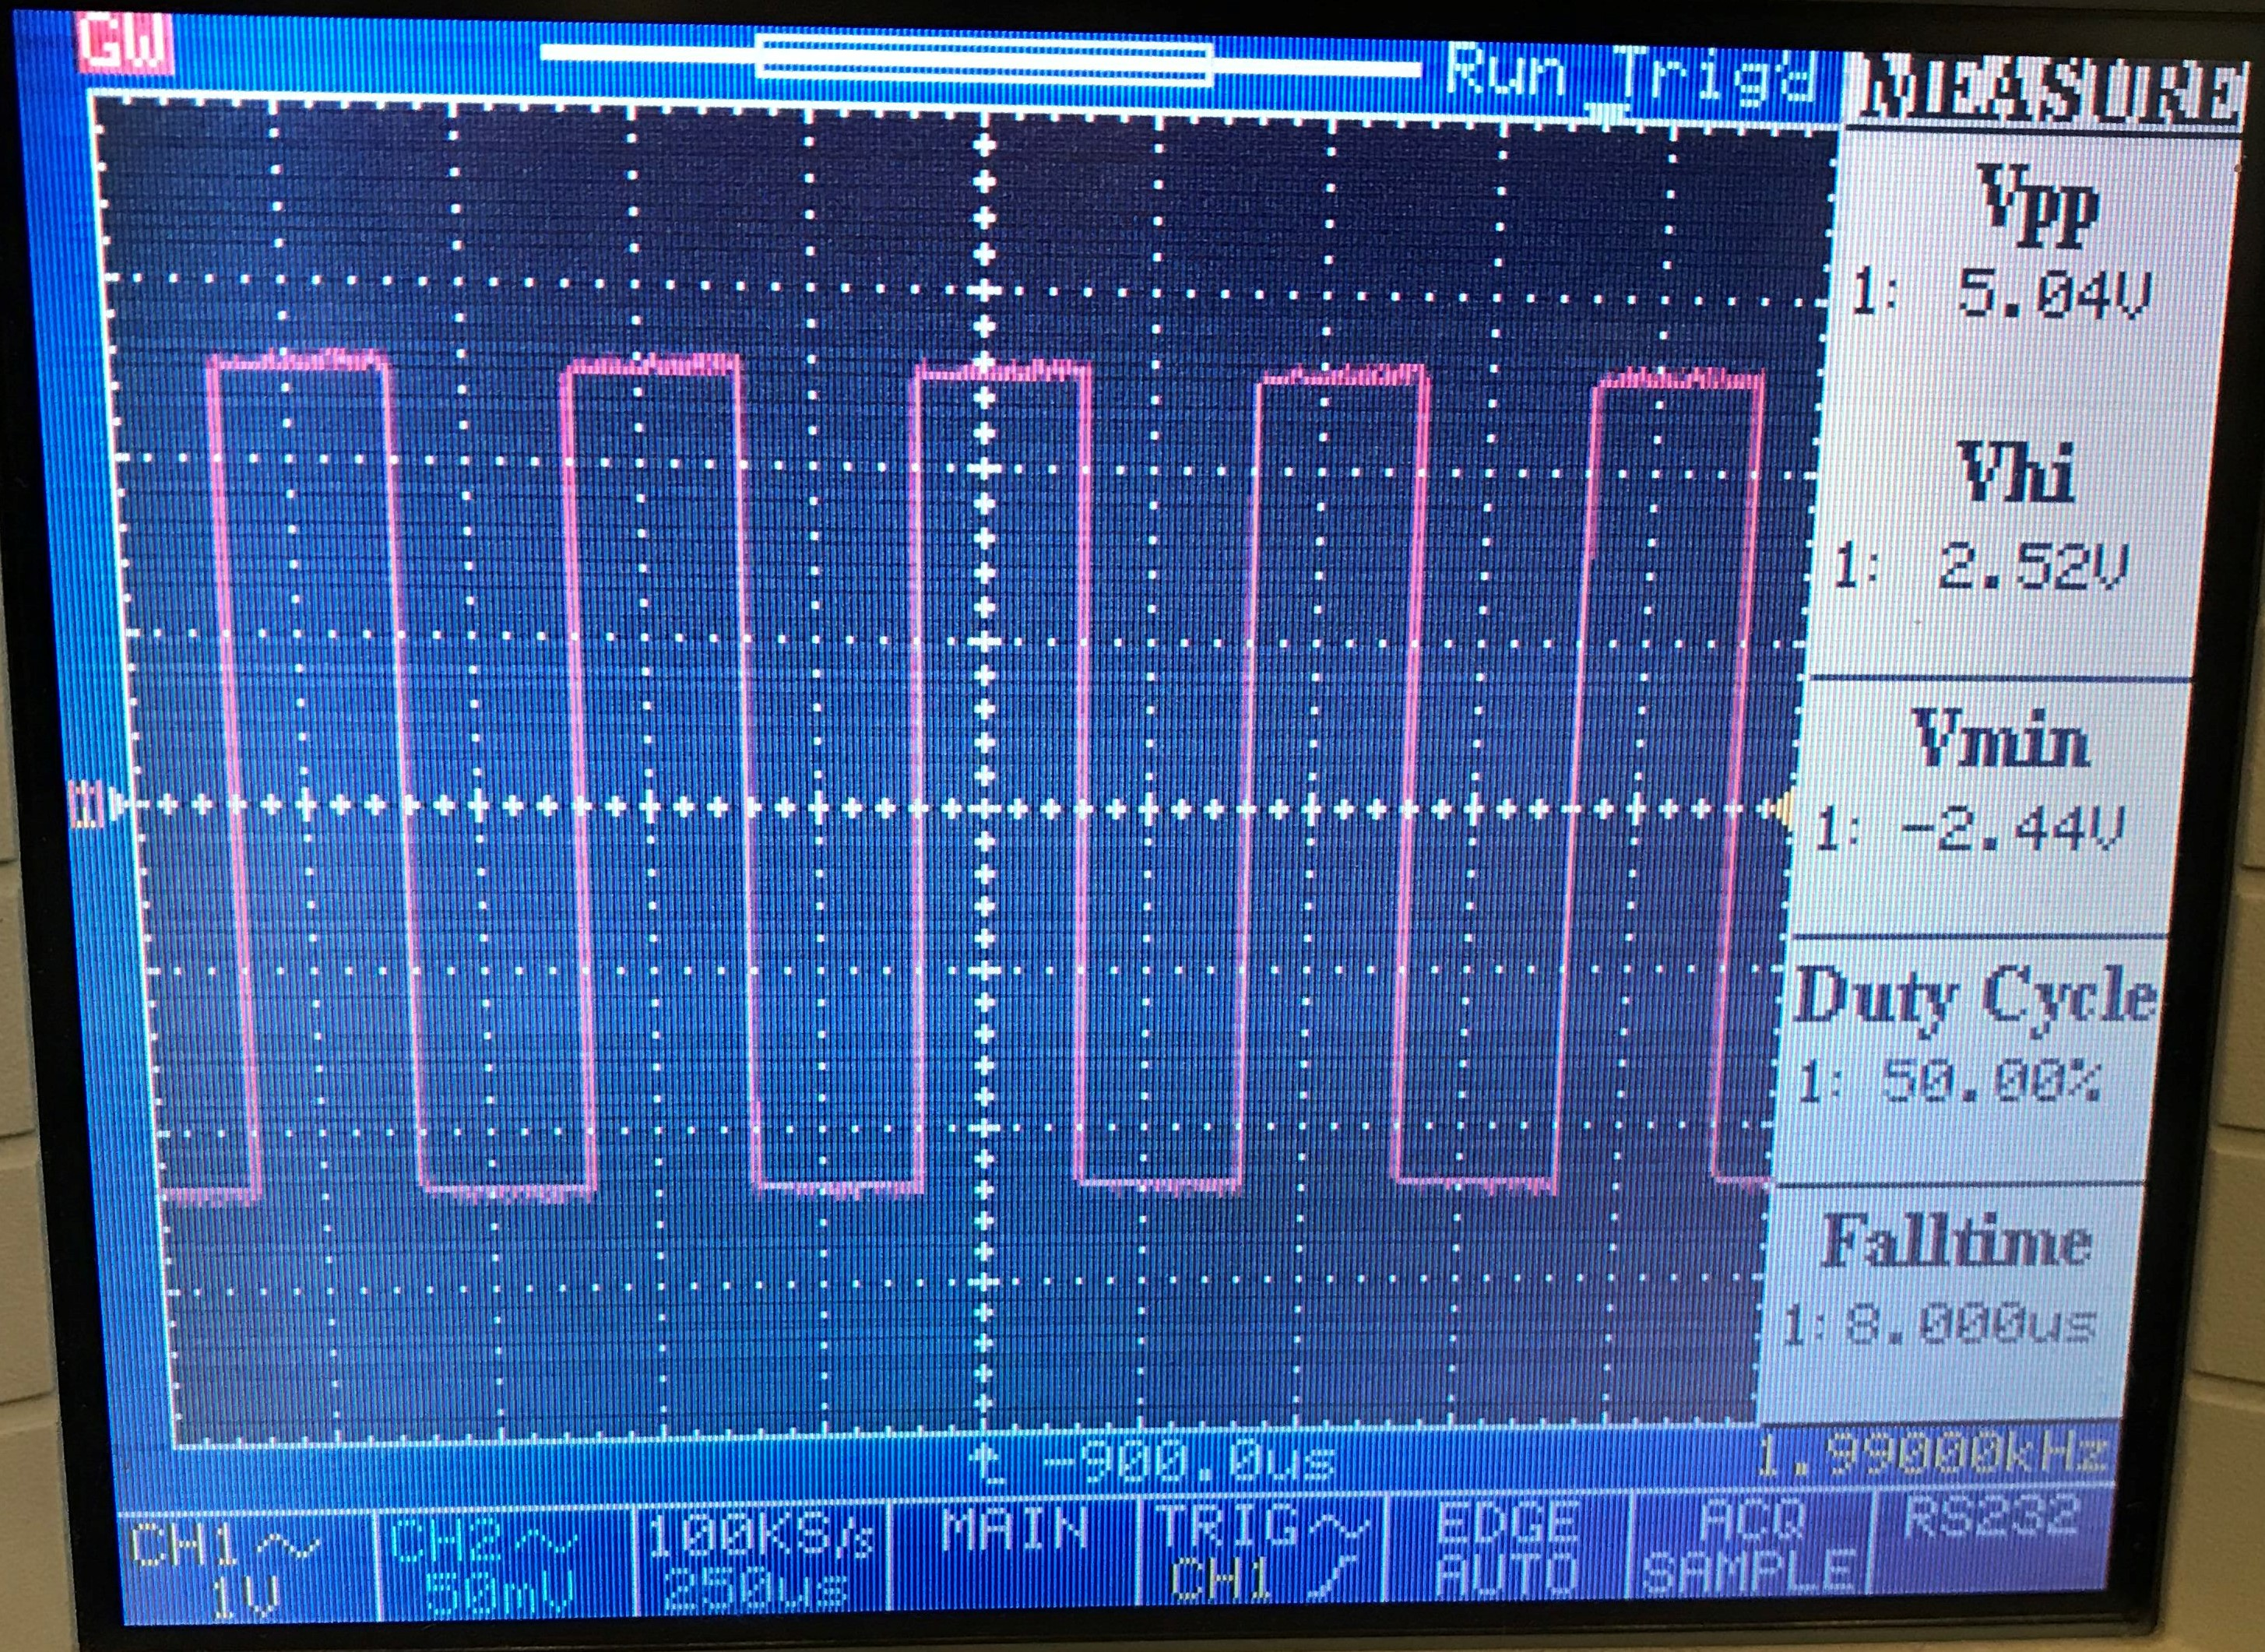
\includegraphics[width=0.5\textwidth]{Photos/5_2_closeup.jpg}
	\caption{5 V (Vpp), 1992 Hz CMOS}
	\label{fig5}
\end{figure}
\paragraph{}
In order to obtain 1992Hz CMOS from the function generator, setting the range selector to 10k and adjusting the voltage was required on CMOS slider. Unlike TTL, CMOS's voltage output can range between 0.6V - 16V.
\end{flushleft}




\begin{flushleft}
\subsubsection{1 V (Vmax), 500 Hz CMOS}
\begin{figure}[h]
    \centering
	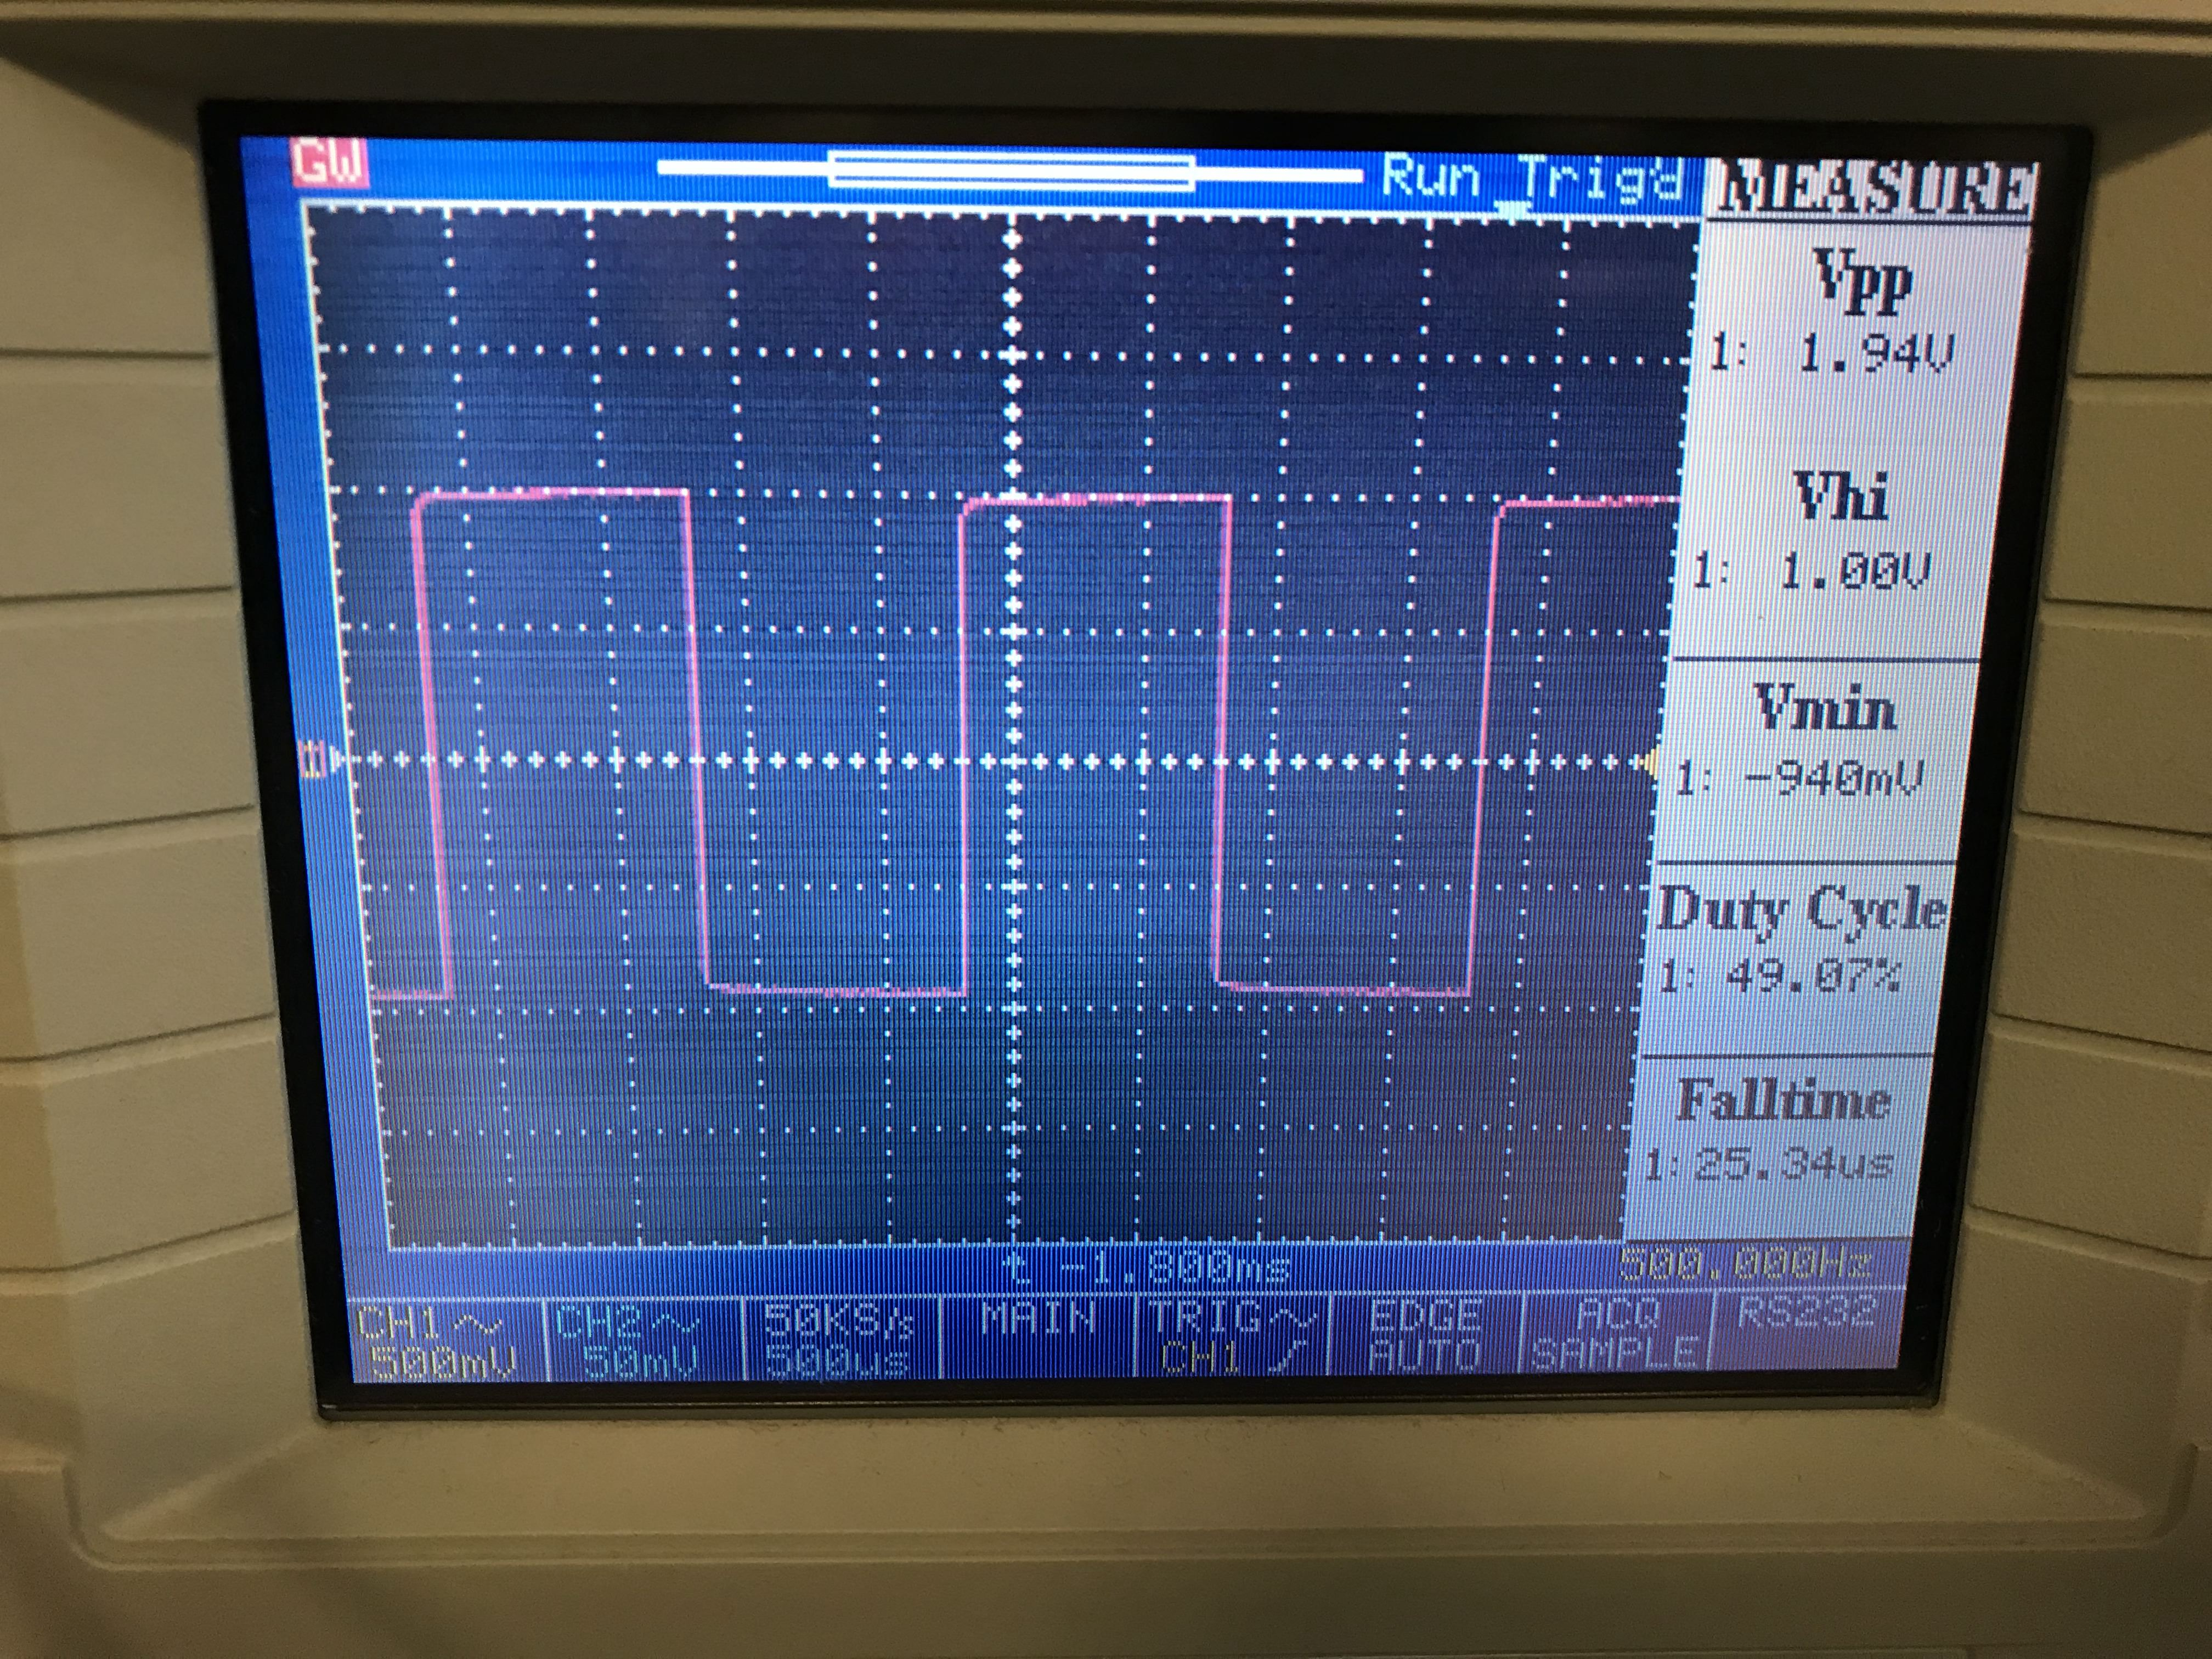
\includegraphics[width=0.5\textwidth]{Photos/5_3_closeup.jpg}
	\caption{1 V (Vmax), 500 Hz CMOS}
	\label{fig6}
\end{figure}
\paragraph{}
In order to obtain 500Hz CMOS from the function generator, maximum frequency was set to 1KHz. 

\end{flushleft}


\newpage
\begin{flushleft}
\subsubsection{3.14 V (Vpp), 0.6 MHz triangular wave}
\begin{figure}[h]
    \centering
	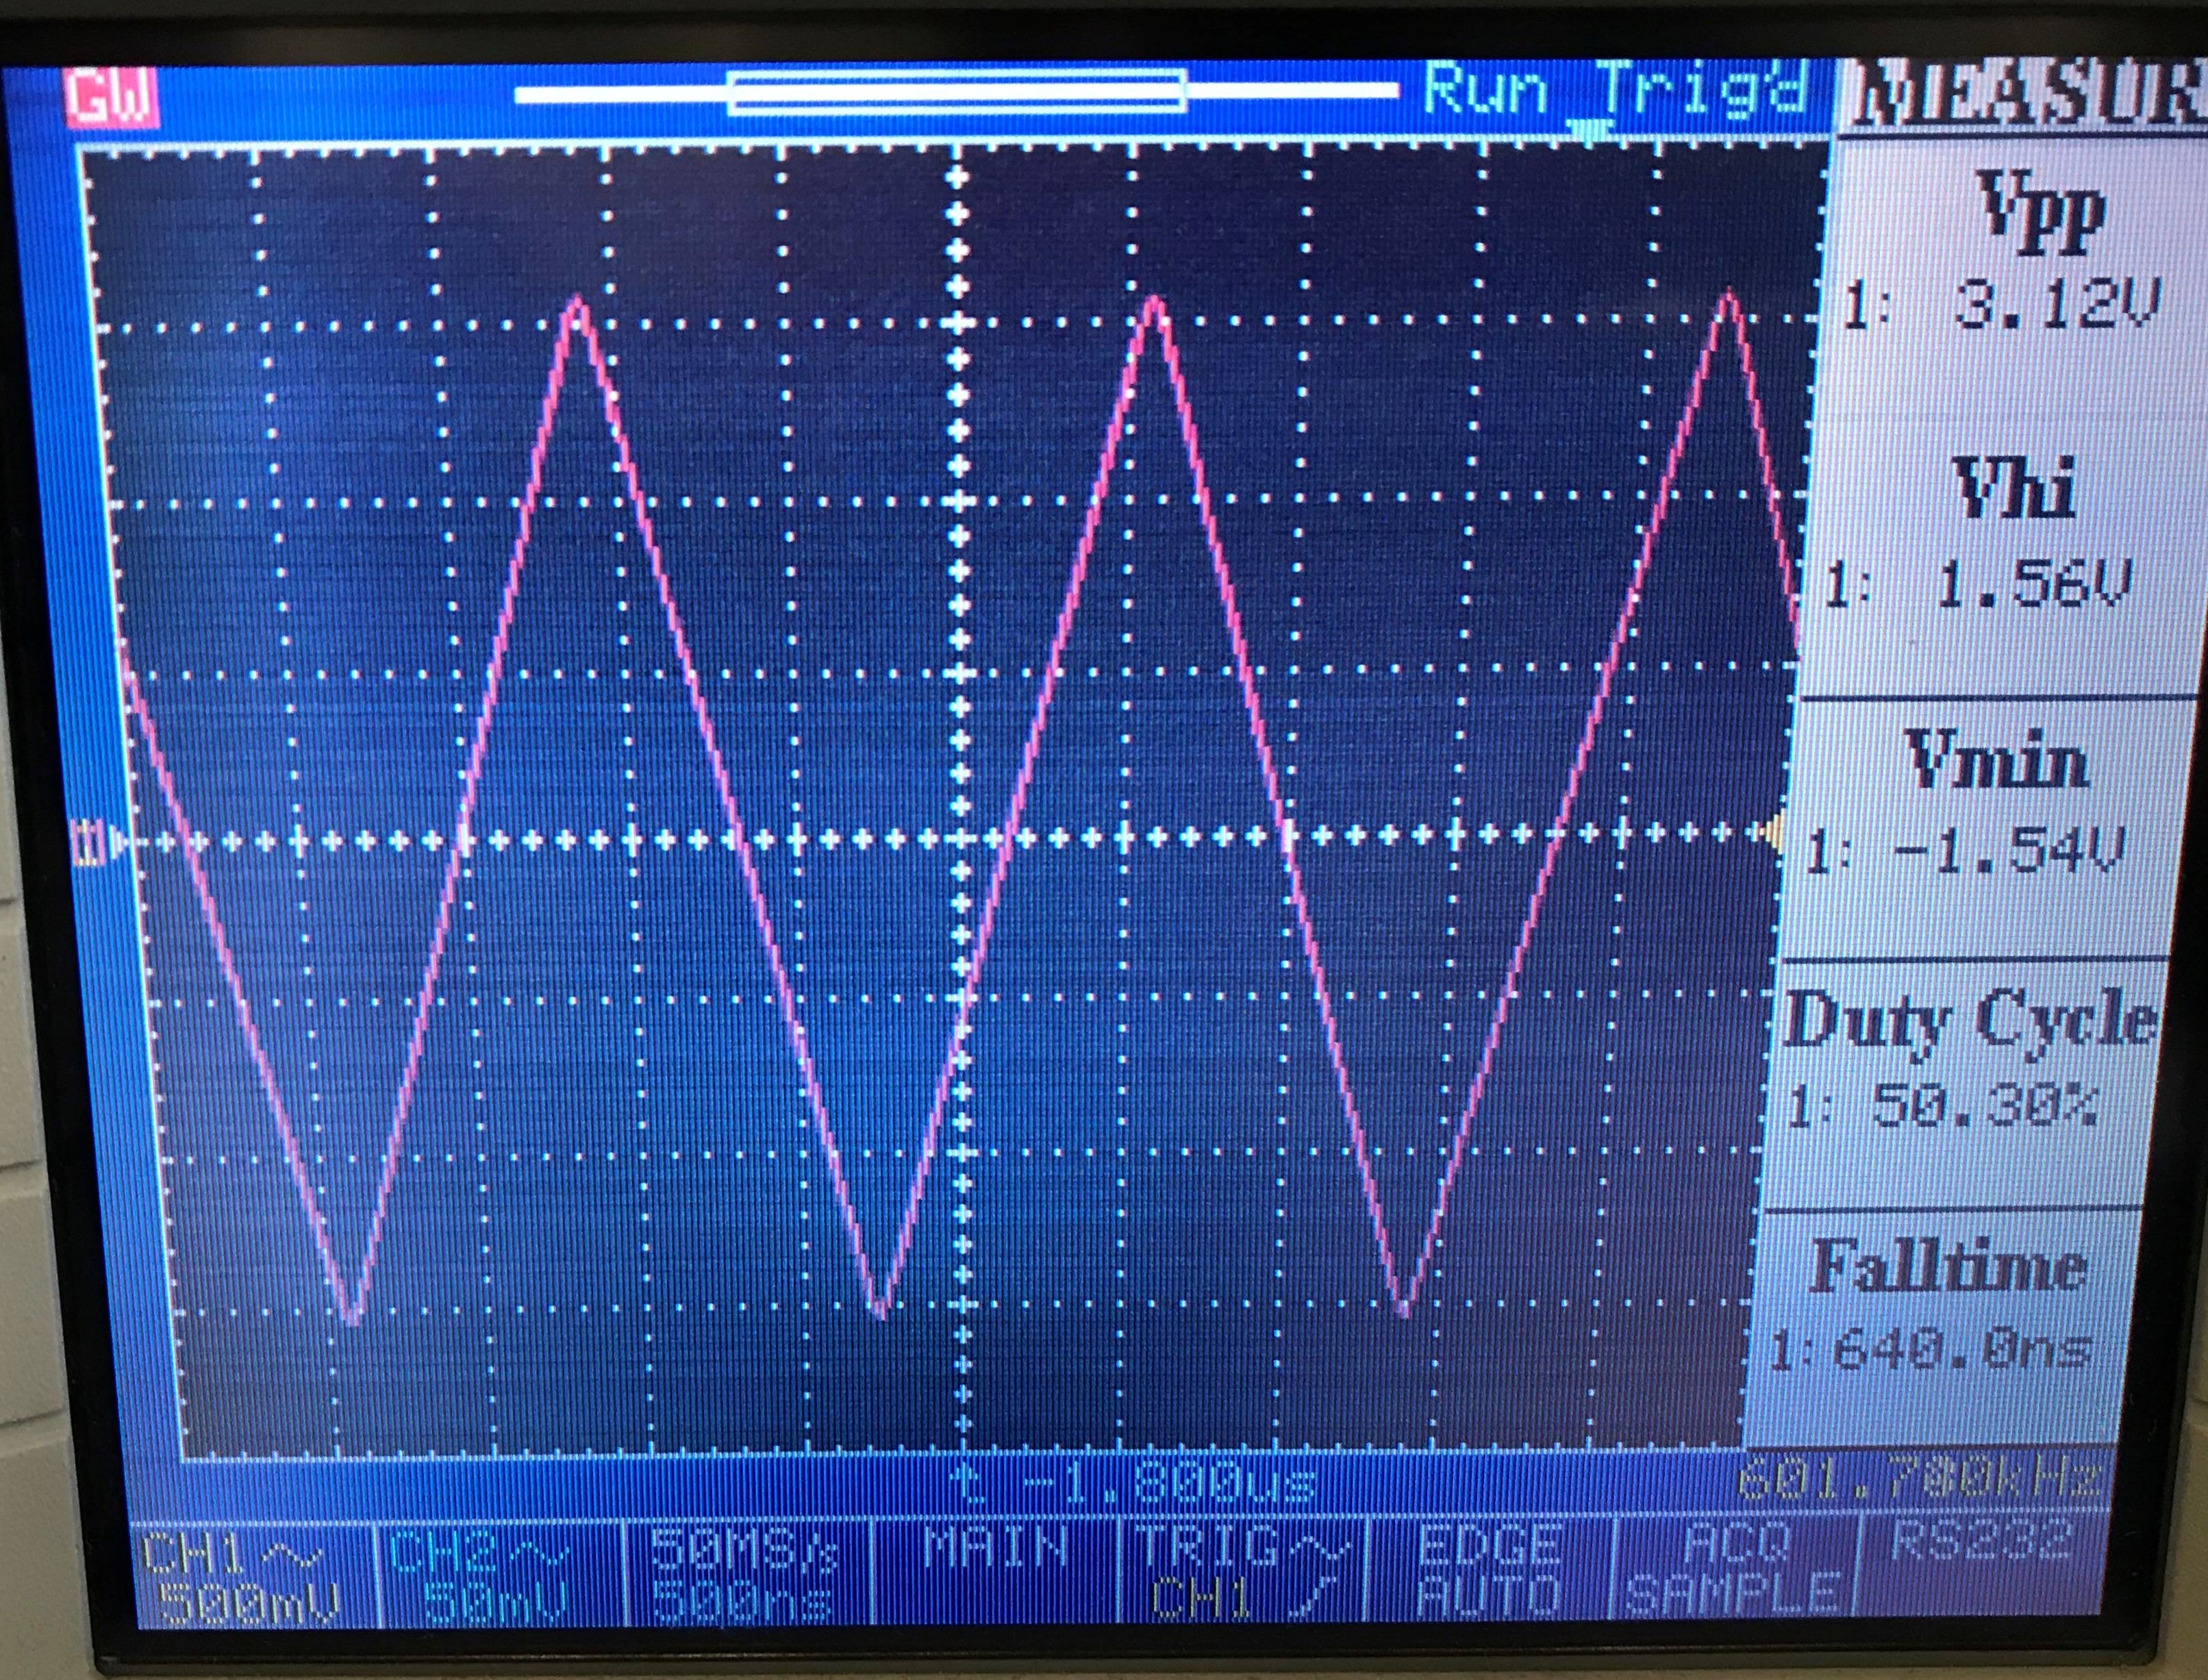
\includegraphics[width=0.5\textwidth]{Photos/5_4_closeup.jpg}
	\caption{3.14 V (Vpp), 0.6 MHz triangular wave}
	\label{fig7}
\end{figure}
\paragraph{}
This time other output of the function generator was used. Which gives you the ability to choose the wave types. Voltage was set to the the value needed and results on the oscilloscope were observed.
\end{flushleft}



\begin{flushleft}
\subsubsection{1.2 V (Vmax), sine wave with 2.5ms period}
\begin{figure}[h]
    \centering
	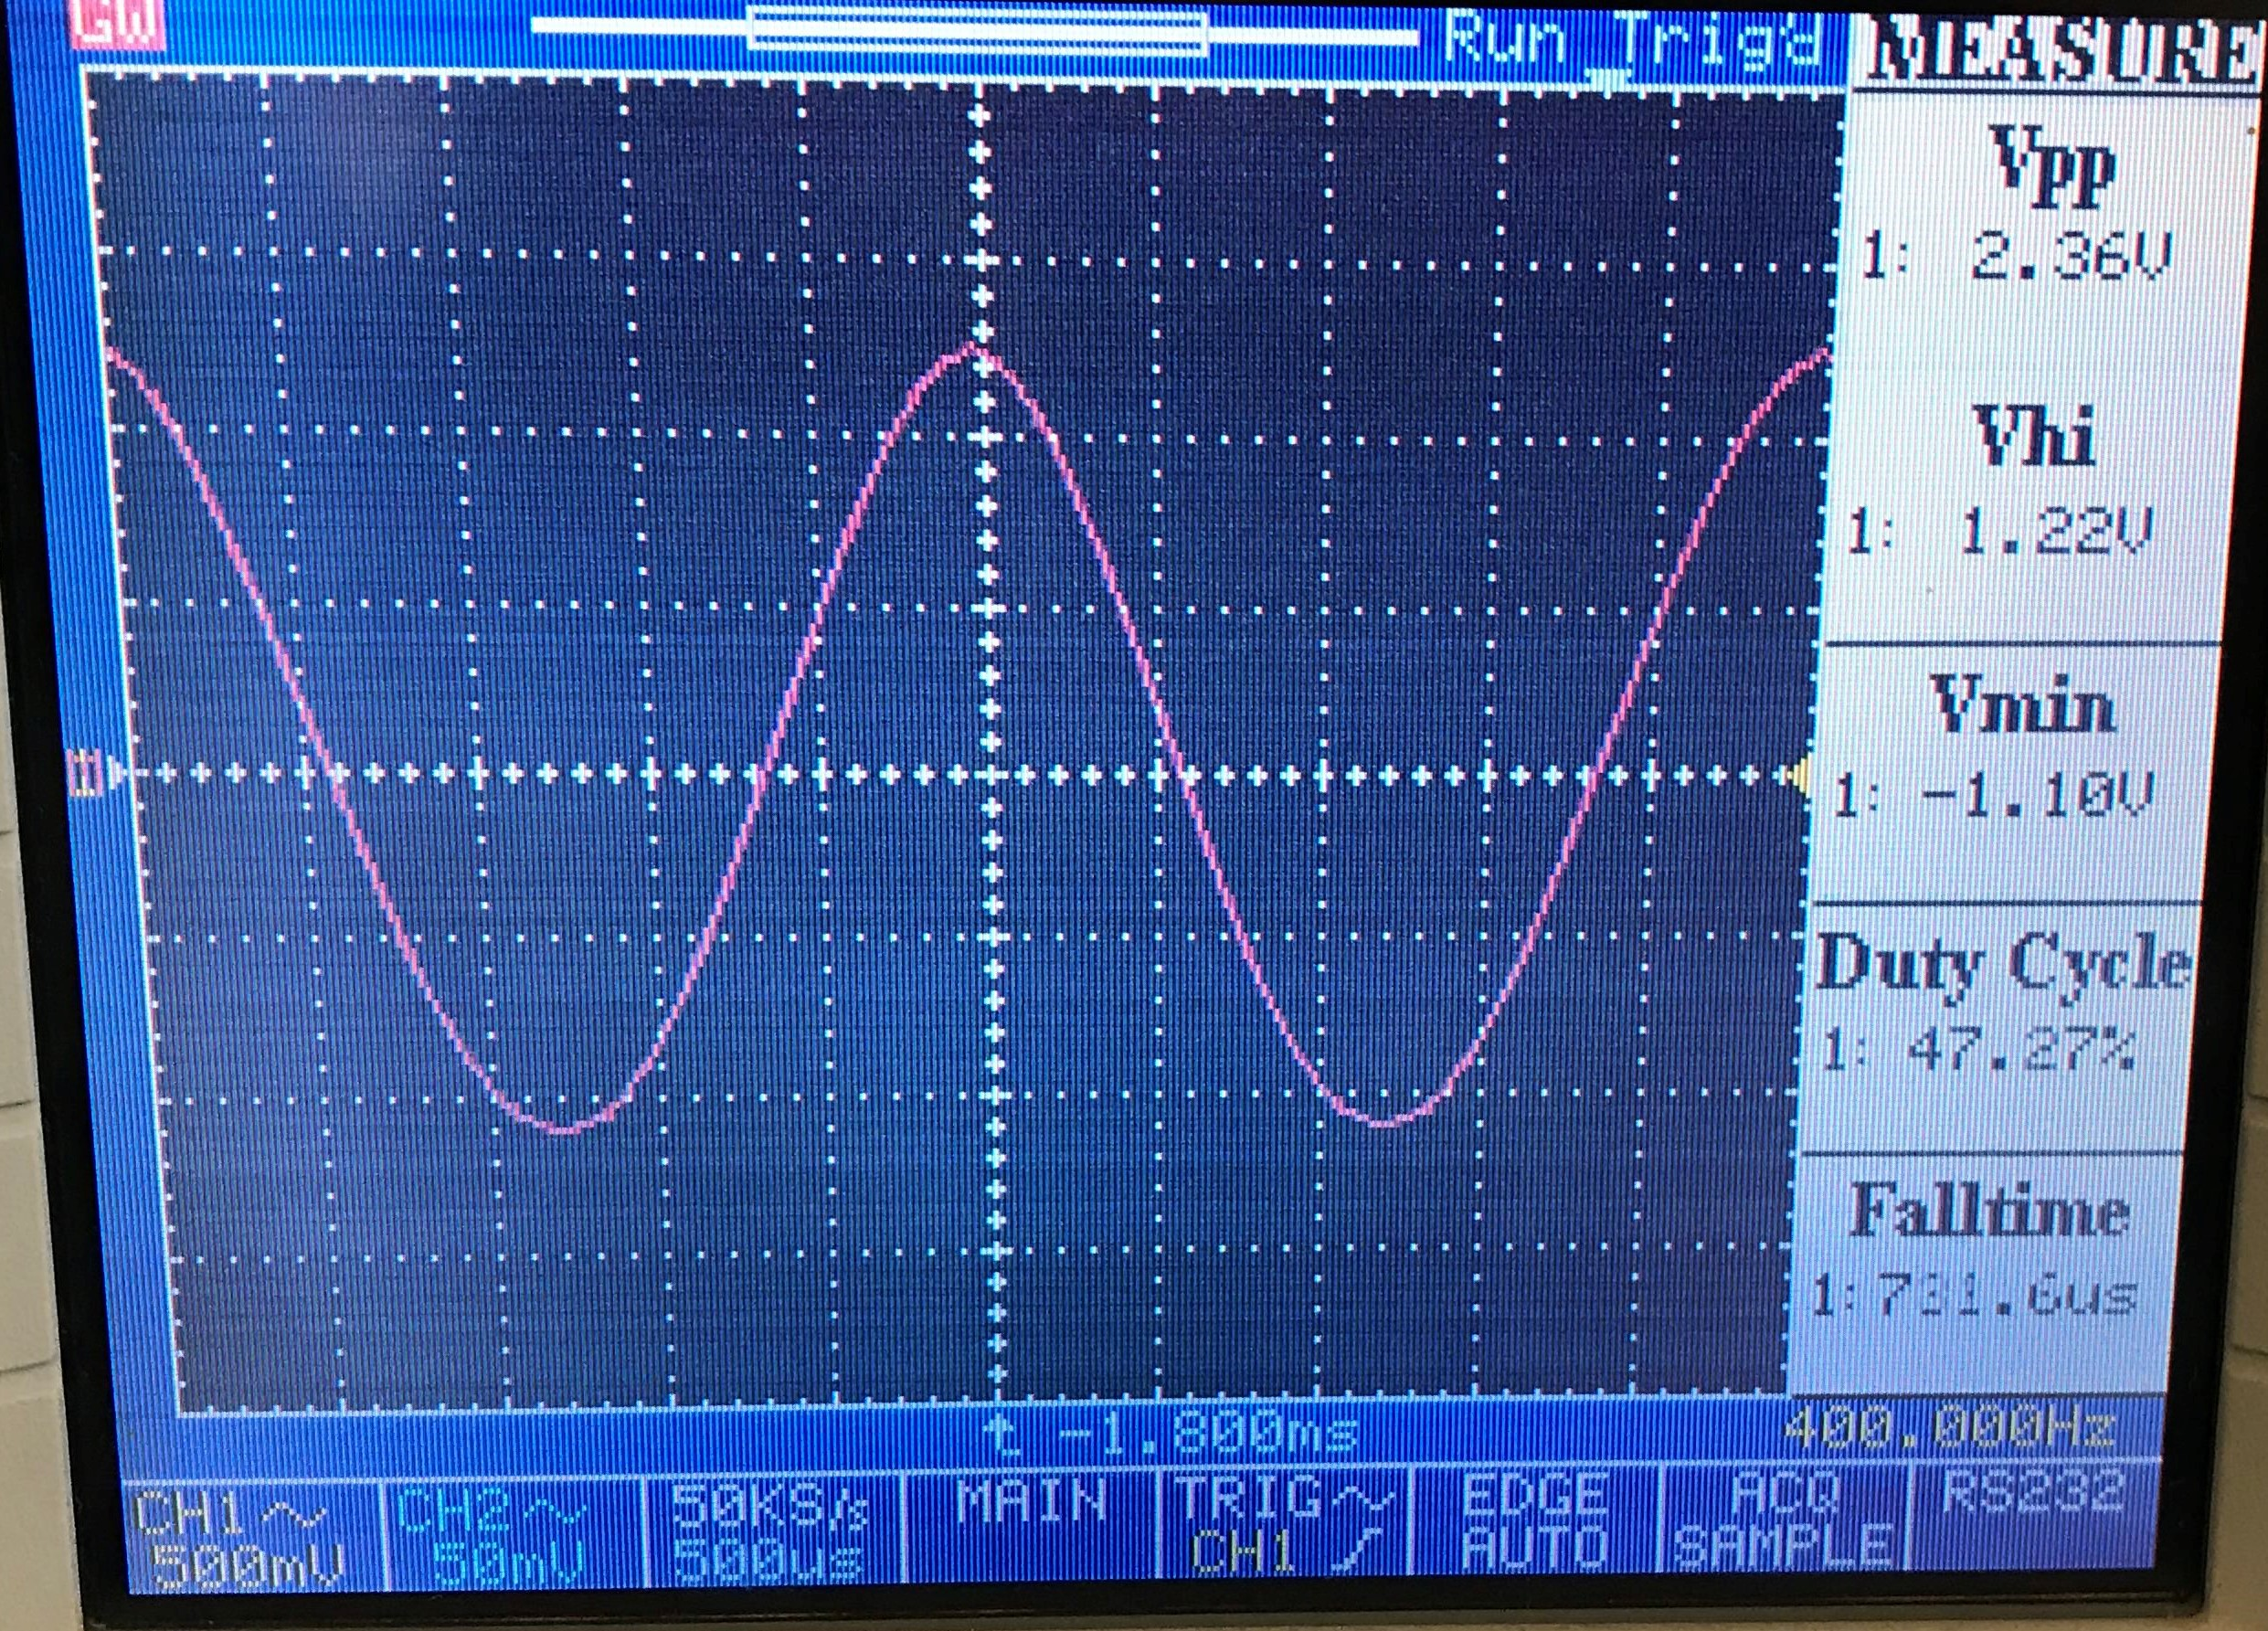
\includegraphics[width=0.5\textwidth]{Photos/5_5_closeup.jpg}
	\caption{1.2 V (Vmax), sine wave with 2.5ms period}
	\label{fig8}
\end{figure}
\paragraph{}
To create a sine wave, we used the same function output as the last one(the one that allows function type selection). Since P= 1/f , frequency had to be 400 Hz. And to get 1.2 Volt Vmax, Vpp was set to 2.4 volts (Due to their relation).
\end{flushleft}



\newpage
\begin{flushleft}
\subsubsection{0.7 V (Vpp), 0.001 GHz square wave}
\begin{figure}[h]
    \centering
	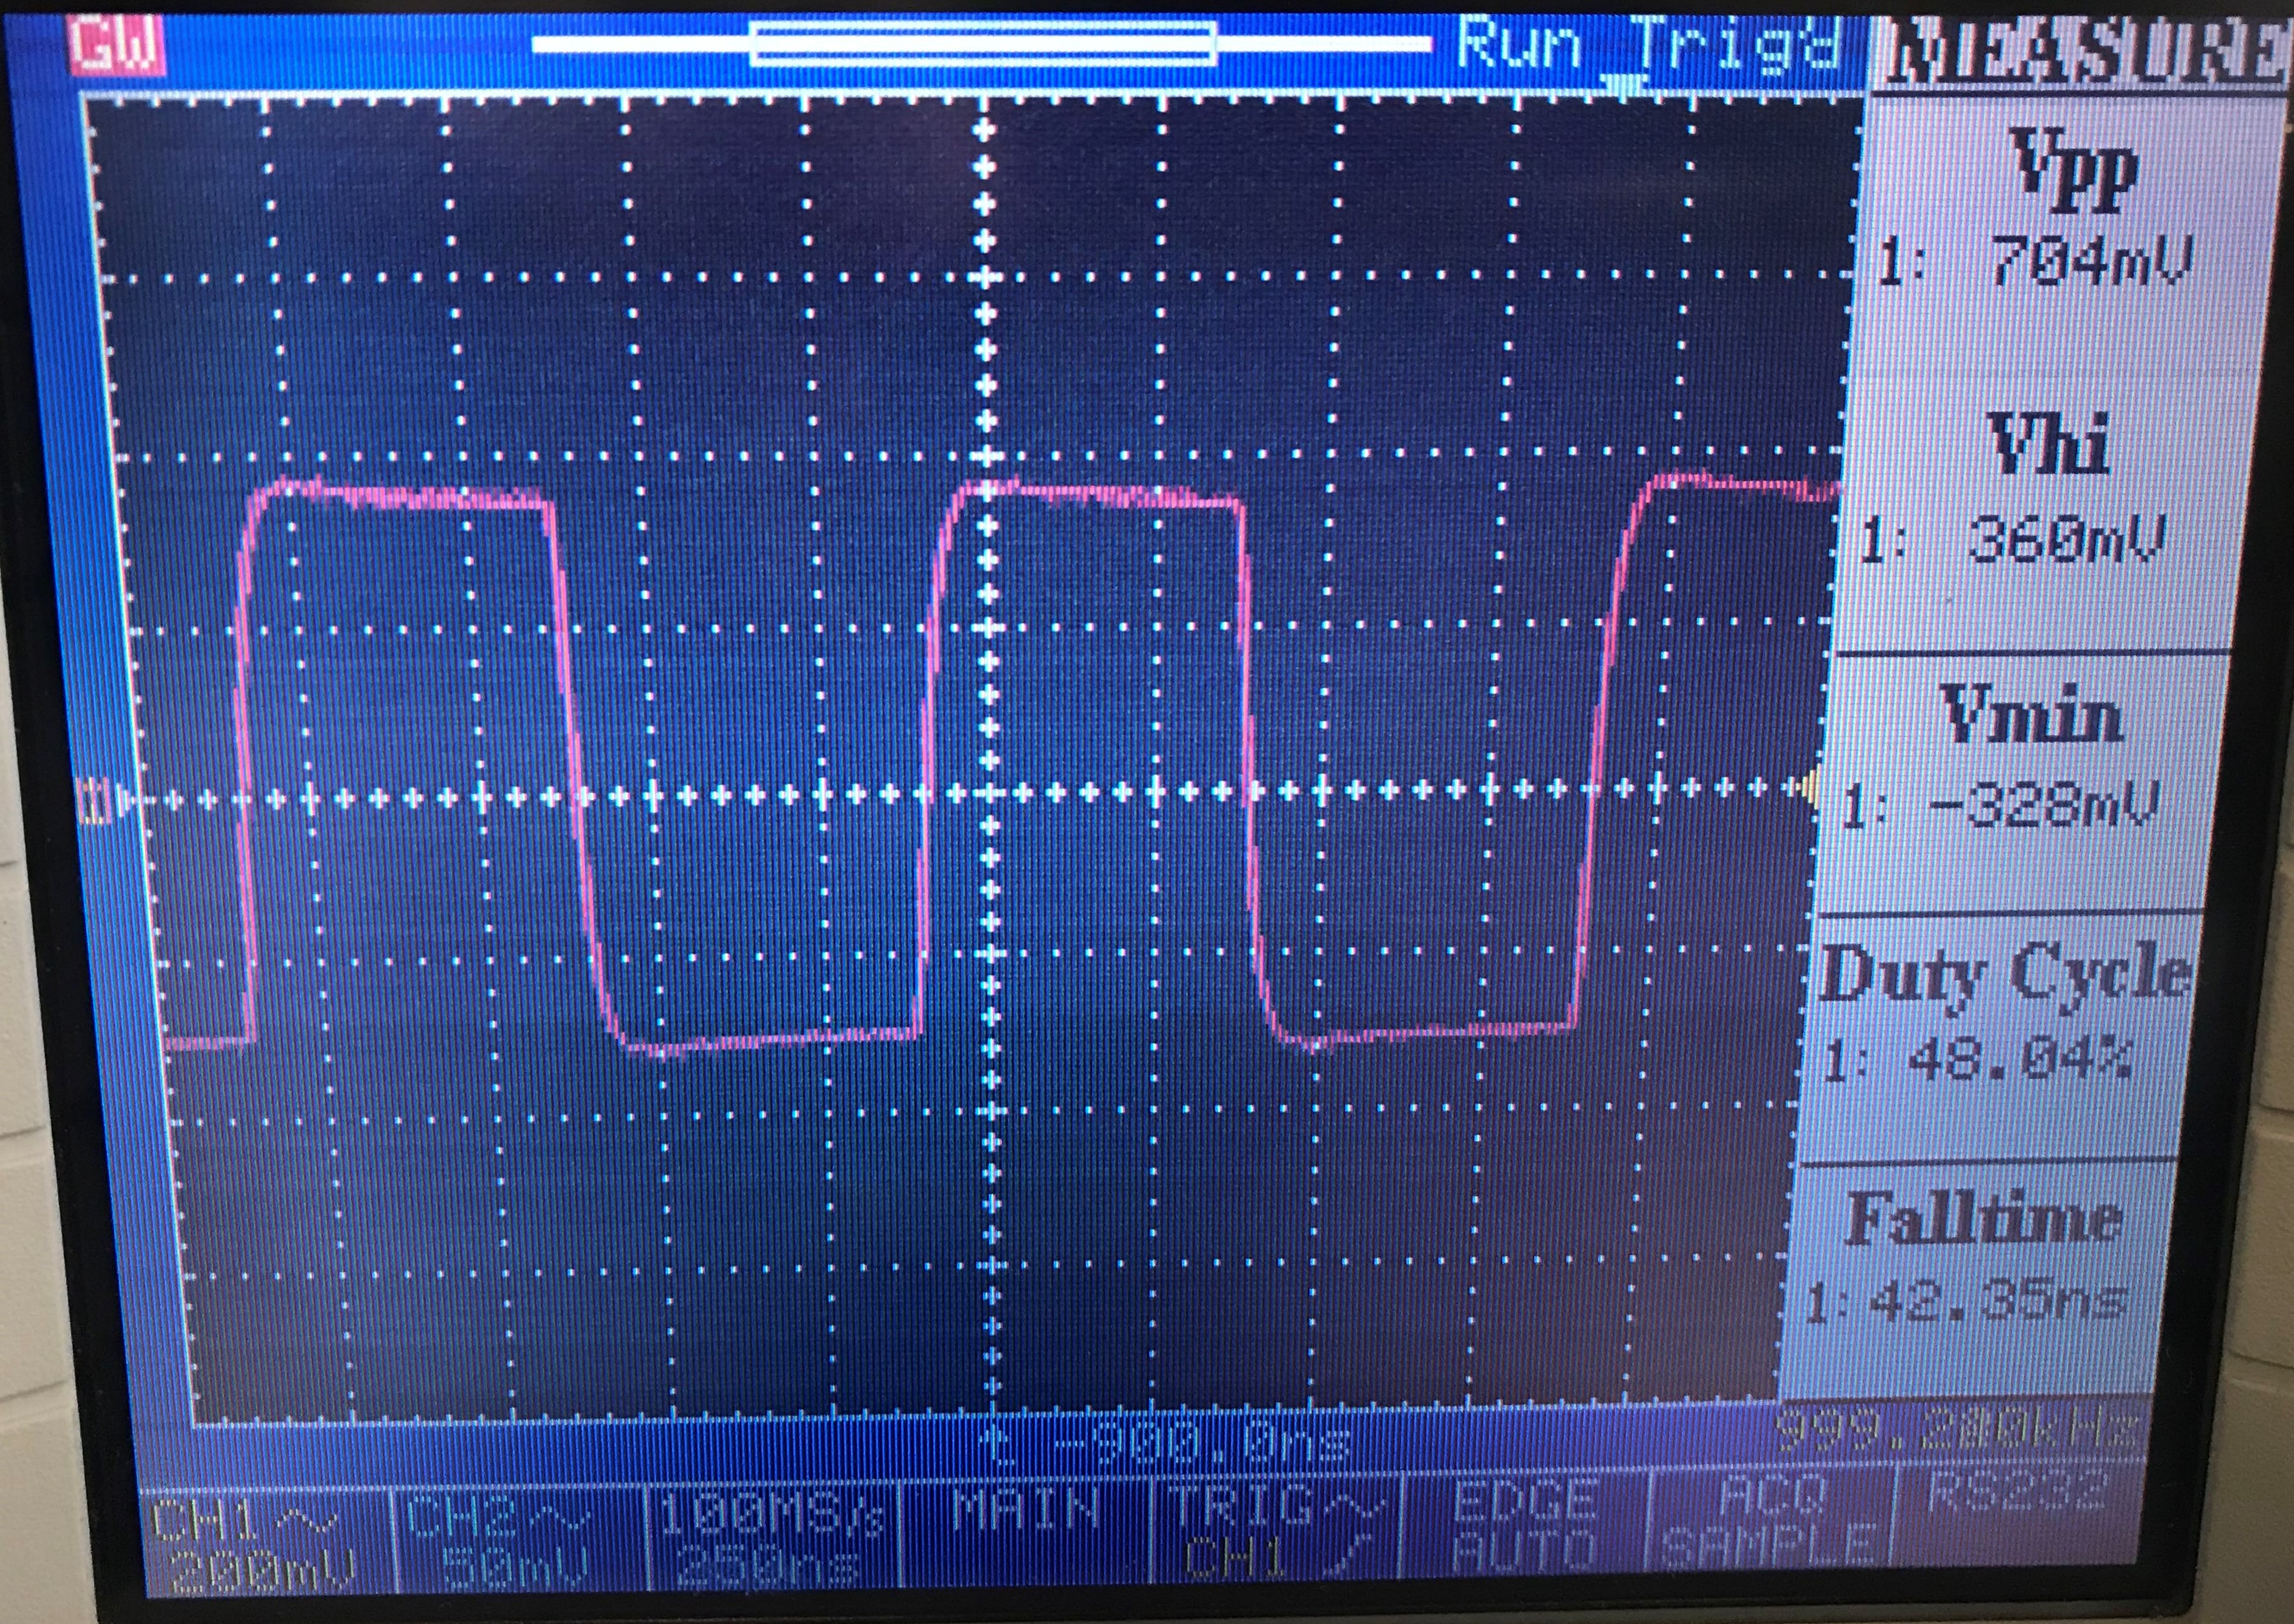
\includegraphics[width=0.5\textwidth]{Photos/5_6_closeup.jpg}
	\caption{0.7 V (Vpp), 0.001 GHz square wave}
	\label{fig9}
\end{figure}

\paragraph{}
Since 0.001 GHz equals to 1 MHz, max frequency was set to 10M for this part. Then Vpp was set to 0.7 volts. To create the square wave we didn't change the output channel, we just changed the output type on the generator to square.

\end{flushleft}



\begin{flushleft}
\subsubsection{1250 mV (Vpp), 45 Hz square wave}
\begin{figure}[h]
    \centering
	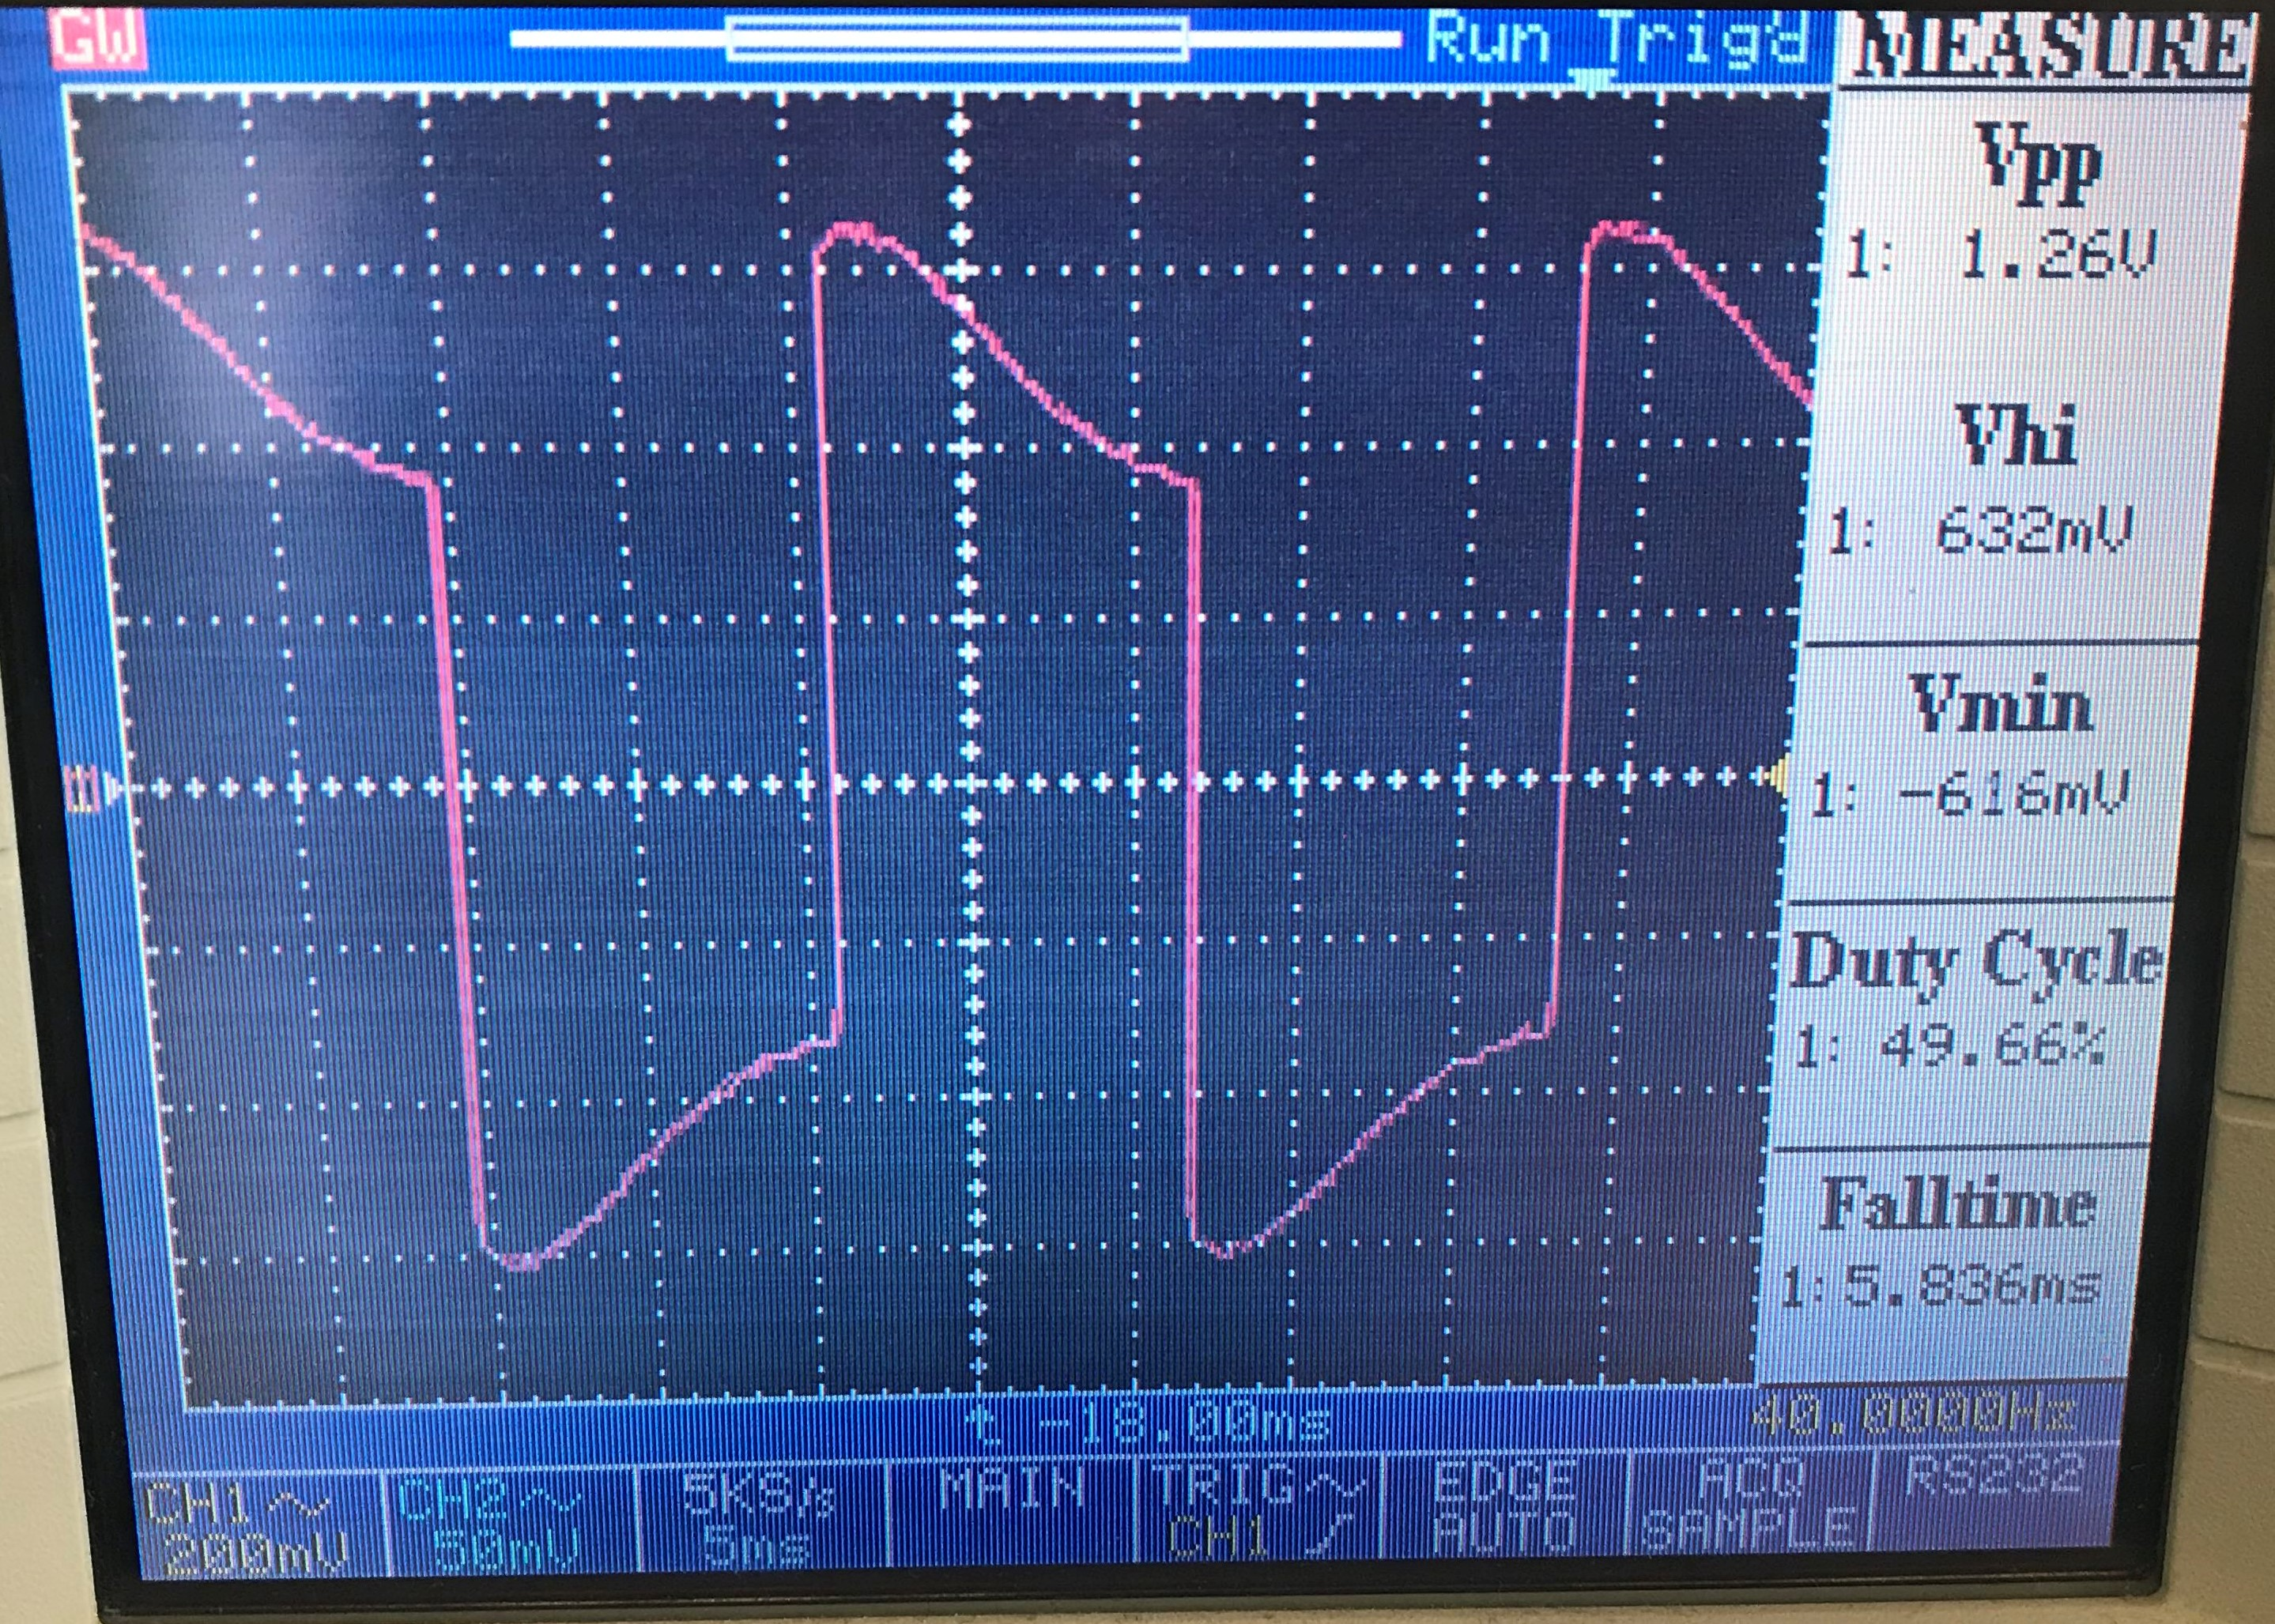
\includegraphics[width=0.5\textwidth]{Photos/5_7_closeup.jpg}
	\caption{1250 mV (Vpp), 45 Hz square wave}
	\label{fig10}
\end{figure}
\paragraph{}
In order to get an input of 1250 mV we had to pull the knob which applies -20db to the output of function generator thus we can have voltage values below 2.4V. As you can see (in Figure 10) waves are not square. Since the frequency is very low, the oscilloscope isn't able to show them properly as they theoretically should look like.
\end{flushleft}




\section{INTERPRETATION OF THE RESULTS}
\begin{flushleft}
\paragraph{}
There weren't many anomalies during the experiments which contradicted with the theoretical results/expectations. In the first 4 parts everything went as planned, as there were no problem with the Vcc and GND values(Differences were close enough to be overlooked) and logic switches on the CADET unit. We were able to observe the theoretically expected results (Monitor lights showing the right values for different voltage values and 74x$x^{1}$04 - Hex Inverter changing monitor results without problem). In part 5, we were able to observe most of the functions which we were supposed to without any errors. However for some of the frequency values couldn't be displayed by the oscilloscope the way they are supposed to look theoretically.
\end{flushleft}

\section{CONCLUSION}
\begin{flushleft}
\paragraph{}
We were able to go through each part without many problems as we finished rather quickly. There were only some minor complications when the function generator was being used. After reading the related parts in the lab booklet once again, we were able to solve those problems pretty easily.  
\end{flushleft}

%\vspace{5mm}
\begin{flushleft}
Things we learned from CADET experiments:
\begin{itemize}
    \item Parts of CADET
    \item SPDT switches allow you to choose both inputs rather than having predetermined values like normal logic switches.
\end{itemize}
\end{flushleft}

%\vspace{5mm}
\begin{flushleft}
\newline Things we learned from function generator/oscilloscope experiments:
\begin{itemize}
    \item TTL is always in form of a square wave while CMOS can be set as different wave types. ( With the function generators in the laboratories that are available to us)
    \item TTL output voltage is fixed to 5 Volts.
    \item CMOS output can be adjusted between 0.6V and 16V.
    \item Vmax is the highest voltage on a wave where Vpp is the difference between highest and lowest points(peak to peak difference).
    % fix these please
\end{itemize}
\end{flushleft}
\newpage
%We learned the power of the AUTO button1

\nocite{overleaf}
\nocite{reportGuide}

\bibliographystyle{unsrt}
\bibliography{reference}

\end{document}

